\documentclass[twoside]{book}

% Packages required by doxygen
\usepackage{calc}
\usepackage{doxygen}
\usepackage{graphicx}
\usepackage[utf8]{inputenc}
\usepackage{makeidx}
\usepackage{multicol}
\usepackage{multirow}
\usepackage{textcomp}
\usepackage[table]{xcolor}

% Font selection
\usepackage[T1]{fontenc}
\usepackage{mathptmx}
\usepackage[scaled=.90]{helvet}
\usepackage{courier}
\usepackage{amssymb}
\usepackage{sectsty}
\renewcommand{\familydefault}{\sfdefault}
\allsectionsfont{%
  \fontseries{bc}\selectfont%
  \color{darkgray}%
}
\renewcommand{\DoxyLabelFont}{%
  \fontseries{bc}\selectfont%
  \color{darkgray}%
}

% Page & text layout
\usepackage{geometry}
\geometry{%
  a4paper,%
  top=2.5cm,%
  bottom=2.5cm,%
  left=2.5cm,%
  right=2.5cm%
}
\tolerance=750
\hfuzz=15pt
\hbadness=750
\setlength{\emergencystretch}{15pt}
\setlength{\parindent}{0cm}
\setlength{\parskip}{0.2cm}
\makeatletter
\renewcommand{\paragraph}{%
  \@startsection{paragraph}{4}{0ex}{-1.0ex}{1.0ex}{%
    \normalfont\normalsize\bfseries\SS@parafont%
  }%
}
\renewcommand{\subparagraph}{%
  \@startsection{subparagraph}{5}{0ex}{-1.0ex}{1.0ex}{%
    \normalfont\normalsize\bfseries\SS@subparafont%
  }%
}
\makeatother

% Headers & footers
\usepackage{fancyhdr}
\pagestyle{fancyplain}
\fancyhead[LE]{\fancyplain{}{\bfseries\thepage}}
\fancyhead[CE]{\fancyplain{}{}}
\fancyhead[RE]{\fancyplain{}{\bfseries\leftmark}}
\fancyhead[LO]{\fancyplain{}{\bfseries\rightmark}}
\fancyhead[CO]{\fancyplain{}{}}
\fancyhead[RO]{\fancyplain{}{\bfseries\thepage}}
\fancyfoot[LE]{\fancyplain{}{}}
\fancyfoot[CE]{\fancyplain{}{}}
\fancyfoot[RE]{\fancyplain{}{\bfseries\scriptsize Generated on Thu Feb 2 2017 05\-:02\-:03 for Laboratorio 0 by Doxygen }}
\fancyfoot[LO]{\fancyplain{}{\bfseries\scriptsize Generated on Thu Feb 2 2017 05\-:02\-:03 for Laboratorio 0 by Doxygen }}
\fancyfoot[CO]{\fancyplain{}{}}
\fancyfoot[RO]{\fancyplain{}{}}
\renewcommand{\footrulewidth}{0.4pt}
\renewcommand{\chaptermark}[1]{%
  \markboth{#1}{}%
}
\renewcommand{\sectionmark}[1]{%
  \markright{\thesection\ #1}%
}

% Indices & bibliography
\usepackage{natbib}
\usepackage[titles]{tocloft}
\setcounter{tocdepth}{3}
\setcounter{secnumdepth}{5}
\makeindex

% Custom commands
\newcommand{\clearemptydoublepage}{%
  \newpage{\pagestyle{empty}\cleardoublepage}%
}


%===== C O N T E N T S =====

\begin{document}

% Titlepage & ToC
\pagenumbering{roman}
\begin{titlepage}
\vspace*{7cm}
\begin{center}%
{\Large Laboratorio 0 }\\
\vspace*{1cm}
{\large Generated by Doxygen 1.8.6}\\
\vspace*{0.5cm}
{\small Thu Feb 2 2017 05:02:03}\\
\end{center}
\end{titlepage}
\clearemptydoublepage
\tableofcontents
\clearemptydoublepage
\pagenumbering{arabic}

%--- Begin generated contents ---
\chapter{Hierarchical Index}
\section{Jerarquía de la clase}
Esta lista de herencias esta ordenada aproximadamente por orden alfabético\-:\begin{DoxyCompactList}
\item \contentsline{section}{Cell$<$ D $>$}{\pageref{class_cell}}{}
\item \contentsline{section}{Cell$<$ string $>$}{\pageref{class_cell}}{}
\item \contentsline{section}{Levenshtein}{\pageref{class_levenshtein}}{}
\item \contentsline{section}{List$<$ D, P $>$}{\pageref{class_list}}{}
\begin{DoxyCompactList}
\item \contentsline{section}{List\-With\-Pointer$<$ D, P $>$}{\pageref{class_list_with_pointer}}{}
\end{DoxyCompactList}
\item \contentsline{section}{List$<$ string, Cell$<$ string $>$ $\ast$ $>$}{\pageref{class_list}}{}
\begin{DoxyCompactList}
\item \contentsline{section}{List\-With\-Pointer$<$ string, Cell$<$ string $>$ $\ast$ $>$}{\pageref{class_list_with_pointer}}{}
\end{DoxyCompactList}
\item \contentsline{section}{Trie}{\pageref{class_trie}}{}
\item \contentsline{section}{Trie\-Node}{\pageref{class_trie_node}}{}
\end{DoxyCompactList}

\chapter{Class Index}
\section{Class List}
Here are the classes, structs, unions and interfaces with brief descriptions\-:\begin{DoxyCompactList}
\item\contentsline{section}{{\bf Animal} }{\pageref{class_animal}}{}
\item\contentsline{section}{{\bf Juego} }{\pageref{class_juego}}{}
\item\contentsline{section}{{\bf Lobo} }{\pageref{class_lobo}}{}
\item\contentsline{section}{{\bf Matriz} }{\pageref{class_matriz}}{}
\item\contentsline{section}{{\bf Oveja} }{\pageref{class_oveja}}{}
\item\contentsline{section}{{\bf Raton} }{\pageref{class_raton}}{}
\item\contentsline{section}{{\bf Zorro} }{\pageref{class_zorro}}{}
\end{DoxyCompactList}

\chapter{File Index}
\section{Lista de archivos}
Lista de todos los archivos documentados y con descripciones breves\-:\begin{DoxyCompactList}
\item\contentsline{section}{{\bfseries Cell.\-h} }{\pageref{_cell_8h}}{}
\item\contentsline{section}{\hyperlink{_levenshtein_8cpp}{Levenshtein.\-cpp} \\*Clase \hyperlink{class_levenshtein}{Levenshtein} }{\pageref{_levenshtein_8cpp}}{}
\item\contentsline{section}{\hyperlink{_levenshtein_8h}{Levenshtein.\-h} \\*Clase \hyperlink{class_levenshtein}{Levenshtein} }{\pageref{_levenshtein_8h}}{}
\item\contentsline{section}{{\bfseries List.\-h} }{\pageref{_list_8h}}{}
\item\contentsline{section}{\hyperlink{_list_with_pointer_8h}{List\-With\-Pointer.\-h} \\*Clase \hyperlink{class_list_with_pointer}{List\-With\-Pointer} }{\pageref{_list_with_pointer_8h}}{}
\item\contentsline{section}{\hyperlink{main_8cpp}{main.\-cpp} \\*Clase main }{\pageref{main_8cpp}}{}
\item\contentsline{section}{\hyperlink{_trie_8cpp}{Trie.\-cpp} \\*Clase \hyperlink{class_trie}{Trie} }{\pageref{_trie_8cpp}}{}
\item\contentsline{section}{\hyperlink{_trie_8h}{Trie.\-h} \\*Clase \hyperlink{class_trie}{Trie} }{\pageref{_trie_8h}}{}
\item\contentsline{section}{\hyperlink{_trie_node_8cpp}{Trie\-Node.\-cpp} \\*Clase \hyperlink{class_trie_node}{Trie\-Node} }{\pageref{_trie_node_8cpp}}{}
\item\contentsline{section}{\hyperlink{_trie_node_8h}{Trie\-Node.\-h} \\*Clase \hyperlink{class_trie_node}{Trie\-Node} }{\pageref{_trie_node_8h}}{}
\end{DoxyCompactList}

\chapter{Class Documentation}
\section{Animal Class Reference}
\label{class_animal}\index{Animal@{Animal}}


{\ttfamily \#include $<$Animal.\-h$>$}



Inheritance diagram for Animal\-:
\nopagebreak
\begin{figure}[H]
\begin{center}
\leavevmode
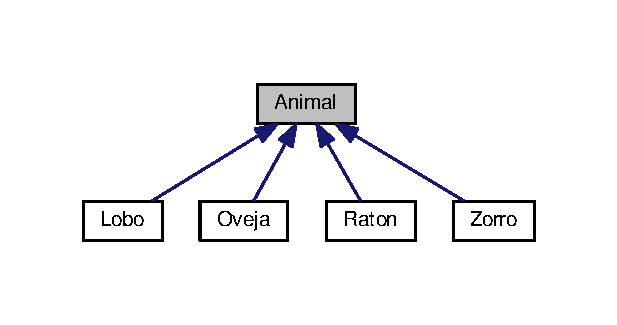
\includegraphics[width=296pt]{class_animal__inherit__graph}
\end{center}
\end{figure}
\subsection*{Public Member Functions}
\begin{DoxyCompactItemize}
\item 
{\bf Animal} ()
\item 
{\bf Animal} (const {\bf Animal} \&orig)
\item 
virtual {\bf $\sim$\-Animal} ()
\item 
string {\bf get\-Sex} ()
\item 
virtual void {\bf operator!} ()=0
\item 
virtual void {\bf operator++} (int)=0
\item 
virtual void {\bf operator$\sim$} ()=0
\item 
virtual void {\bf operator-\/-\/} (int)=0
\item 
virtual void {\bf macho\-Alfa} ()=0
\item 
int $\ast$ {\bf buscar} (string busq)
\item 
int $\ast$ {\bf get\-Espacio} ()
\end{DoxyCompactItemize}
\subsection*{Public Attributes}
\begin{DoxyCompactItemize}
\item 
int {\bf energia}
\item 
string {\bf identificador}
\item 
string {\bf sexo}
\item 
string {\bf especie}
\item 
int {\bf ubicacion} [2]
\item 
bool {\bf se\-Reprodujo}
\item 
bool {\bf se\-Movio}
\end{DoxyCompactItemize}


\subsection{Constructor \& Destructor Documentation}
\index{Animal@{Animal}!Animal@{Animal}}
\index{Animal@{Animal}!Animal@{Animal}}
\subsubsection[{Animal}]{\setlength{\rightskip}{0pt plus 5cm}Animal\-::\-Animal (
\begin{DoxyParamCaption}
{}
\end{DoxyParamCaption}
)}\label{class_animal_a1e726a49ec952443190ac62dad22353c}
\index{Animal@{Animal}!Animal@{Animal}}
\index{Animal@{Animal}!Animal@{Animal}}
\subsubsection[{Animal}]{\setlength{\rightskip}{0pt plus 5cm}Animal\-::\-Animal (
\begin{DoxyParamCaption}
\item[{const {\bf Animal} \&}]{orig}
\end{DoxyParamCaption}
)}\label{class_animal_ab26f5f62b5194201e0b07729bde2f5dc}
\index{Animal@{Animal}!$\sim$\-Animal@{$\sim$\-Animal}}
\index{$\sim$\-Animal@{$\sim$\-Animal}!Animal@{Animal}}
\subsubsection[{$\sim$\-Animal}]{\setlength{\rightskip}{0pt plus 5cm}Animal\-::$\sim$\-Animal (
\begin{DoxyParamCaption}
{}
\end{DoxyParamCaption}
)\hspace{0.3cm}{\ttfamily [virtual]}}\label{class_animal_a476af25adde5f0dfa688129c8f86fa5c}


\subsection{Member Function Documentation}
\index{Animal@{Animal}!buscar@{buscar}}
\index{buscar@{buscar}!Animal@{Animal}}
\subsubsection[{buscar}]{\setlength{\rightskip}{0pt plus 5cm}int $\ast$ Animal\-::buscar (
\begin{DoxyParamCaption}
\item[{string}]{busq}
\end{DoxyParamCaption}
)}\label{class_animal_a8676b59bee05f46ad2a57c372933359c}


Here is the caller graph for this function\-:
\nopagebreak
\begin{figure}[H]
\begin{center}
\leavevmode
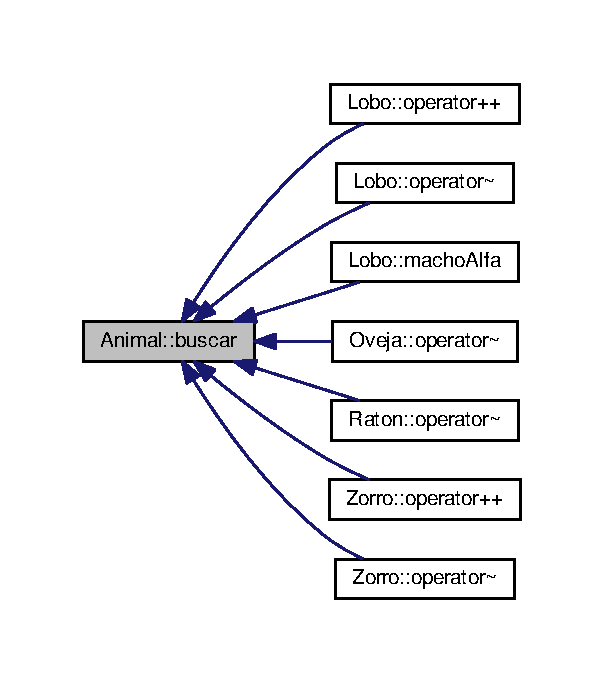
\includegraphics[width=290pt]{class_animal_a8676b59bee05f46ad2a57c372933359c_icgraph}
\end{center}
\end{figure}


\index{Animal@{Animal}!get\-Espacio@{get\-Espacio}}
\index{get\-Espacio@{get\-Espacio}!Animal@{Animal}}
\subsubsection[{get\-Espacio}]{\setlength{\rightskip}{0pt plus 5cm}int $\ast$ Animal\-::get\-Espacio (
\begin{DoxyParamCaption}
{}
\end{DoxyParamCaption}
)}\label{class_animal_a89fe9c1774986a838d83217464d58b1f}


Here is the caller graph for this function\-:
\nopagebreak
\begin{figure}[H]
\begin{center}
\leavevmode
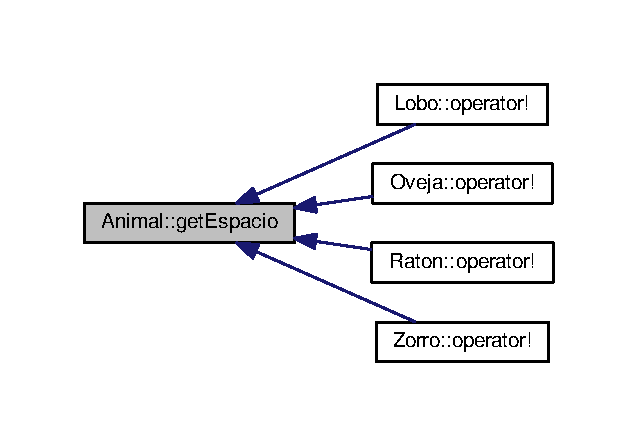
\includegraphics[width=306pt]{class_animal_a89fe9c1774986a838d83217464d58b1f_icgraph}
\end{center}
\end{figure}


\index{Animal@{Animal}!get\-Sex@{get\-Sex}}
\index{get\-Sex@{get\-Sex}!Animal@{Animal}}
\subsubsection[{get\-Sex}]{\setlength{\rightskip}{0pt plus 5cm}string Animal\-::get\-Sex (
\begin{DoxyParamCaption}
{}
\end{DoxyParamCaption}
)}\label{class_animal_ae1626c6c4eb5585eaf18df9bf9bb0e01}


Here is the caller graph for this function\-:
\nopagebreak
\begin{figure}[H]
\begin{center}
\leavevmode
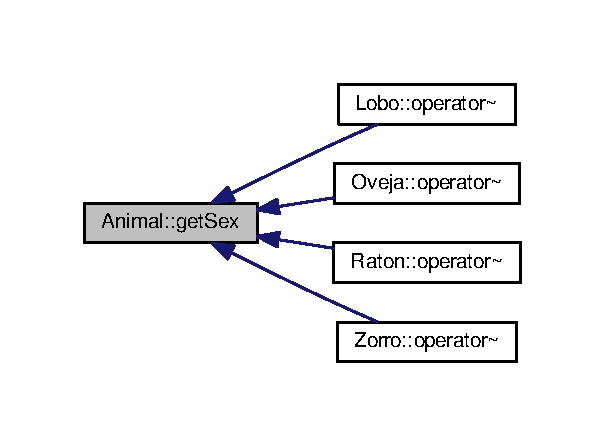
\includegraphics[width=290pt]{class_animal_ae1626c6c4eb5585eaf18df9bf9bb0e01_icgraph}
\end{center}
\end{figure}


\index{Animal@{Animal}!macho\-Alfa@{macho\-Alfa}}
\index{macho\-Alfa@{macho\-Alfa}!Animal@{Animal}}
\subsubsection[{macho\-Alfa}]{\setlength{\rightskip}{0pt plus 5cm}virtual void Animal\-::macho\-Alfa (
\begin{DoxyParamCaption}
{}
\end{DoxyParamCaption}
)\hspace{0.3cm}{\ttfamily [pure virtual]}}\label{class_animal_af0195b0b3cec650e1ece60edd6e031ef}


Implemented in {\bf Raton} \doxyref{}{p.}{class_raton_a6b74bd921ef203b600be27e9c28a14c8}, {\bf Zorro} \doxyref{}{p.}{class_zorro_af1ca7e321452975225376d77905b4a5b}, {\bf Oveja} \doxyref{}{p.}{class_oveja_a7821f1605ff38842fac3d79d3ad534c6}, and {\bf Lobo} \doxyref{}{p.}{class_lobo_a50dac66859d049bc94d0d741297bae3c}.

\index{Animal@{Animal}!operator!@{operator!}}
\index{operator!@{operator!}!Animal@{Animal}}
\subsubsection[{operator!}]{\setlength{\rightskip}{0pt plus 5cm}virtual void Animal\-::operator! (
\begin{DoxyParamCaption}
{}
\end{DoxyParamCaption}
)\hspace{0.3cm}{\ttfamily [pure virtual]}}\label{class_animal_a0def749264daf97160df081b0c028ffe}


Implemented in {\bf Raton} \doxyref{}{p.}{class_raton_a7d07f8b6493b3ee9130ba0143acd755f}, {\bf Zorro} \doxyref{}{p.}{class_zorro_ab9ddecca664da566680332b0aa0ba225}, {\bf Oveja} \doxyref{}{p.}{class_oveja_ae63ca7bb074bf36591e3f12f2c7a9037}, and {\bf Lobo} \doxyref{}{p.}{class_lobo_a3d93cb16a5a0f1e93e0321116227ac14}.

\index{Animal@{Animal}!operator++@{operator++}}
\index{operator++@{operator++}!Animal@{Animal}}
\subsubsection[{operator++}]{\setlength{\rightskip}{0pt plus 5cm}virtual void Animal\-::operator++ (
\begin{DoxyParamCaption}
\item[{int}]{}
\end{DoxyParamCaption}
)\hspace{0.3cm}{\ttfamily [pure virtual]}}\label{class_animal_a82bc2c40b773a232548f961053f9067d}


Implemented in {\bf Raton} \doxyref{}{p.}{class_raton_acd6d6d7e944c9212e368dab9ffb32b72}, {\bf Zorro} \doxyref{}{p.}{class_zorro_a747bf931fd26445891eb3af3785a0356}, {\bf Oveja} \doxyref{}{p.}{class_oveja_a80f81a1a32548bcec1e1b28ea5f9b503}, and {\bf Lobo} \doxyref{}{p.}{class_lobo_a49fcb341d6af488987d7c8a10ad45b38}.

\index{Animal@{Animal}!operator-\/-\/@{operator-\/-\/}}
\index{operator-\/-\/@{operator-\/-\/}!Animal@{Animal}}
\subsubsection[{operator-\/-\/}]{\setlength{\rightskip}{0pt plus 5cm}virtual void Animal\-::operator-\/-\/ (
\begin{DoxyParamCaption}
\item[{int}]{}
\end{DoxyParamCaption}
)\hspace{0.3cm}{\ttfamily [pure virtual]}}\label{class_animal_a43d005a7b5dfa9888a9db21e1e864609}


Implemented in {\bf Raton} \doxyref{}{p.}{class_raton_ac6c595aae5f66043f2e3cce1dd38e0e0}, {\bf Zorro} \doxyref{}{p.}{class_zorro_ac6abad94a814d37f66f6a7698c75493e}, {\bf Oveja} \doxyref{}{p.}{class_oveja_a3cc9887909aeb093a1133f48d6c13670}, and {\bf Lobo} \doxyref{}{p.}{class_lobo_a880e124e43304deac3aa16188ed7fec6}.

\index{Animal@{Animal}!operator$\sim$@{operator$\sim$}}
\index{operator$\sim$@{operator$\sim$}!Animal@{Animal}}
\subsubsection[{operator$\sim$}]{\setlength{\rightskip}{0pt plus 5cm}virtual void Animal\-::operator$\sim$ (
\begin{DoxyParamCaption}
{}
\end{DoxyParamCaption}
)\hspace{0.3cm}{\ttfamily [pure virtual]}}\label{class_animal_a6539ec18d8975982b65de76d8e5638f0}


Implemented in {\bf Raton} \doxyref{}{p.}{class_raton_a7ec71ea95a98d13bf2cccf108b3c76d6}, {\bf Zorro} \doxyref{}{p.}{class_zorro_a9fdef26a109d506ac85b739c9920cc85}, {\bf Oveja} \doxyref{}{p.}{class_oveja_a0ff5ac43f8a666b3b130de88da605fe2}, and {\bf Lobo} \doxyref{}{p.}{class_lobo_a2b4bba4b6d6efa24af4d8e3b986dc7f2}.



\subsection{Member Data Documentation}
\index{Animal@{Animal}!energia@{energia}}
\index{energia@{energia}!Animal@{Animal}}
\subsubsection[{energia}]{\setlength{\rightskip}{0pt plus 5cm}int Animal\-::energia}\label{class_animal_a2a0fbd8a45d845982fa527c76e336084}
\index{Animal@{Animal}!especie@{especie}}
\index{especie@{especie}!Animal@{Animal}}
\subsubsection[{especie}]{\setlength{\rightskip}{0pt plus 5cm}string Animal\-::especie}\label{class_animal_a6d08af00ece2985d73126798973f84a8}
\index{Animal@{Animal}!identificador@{identificador}}
\index{identificador@{identificador}!Animal@{Animal}}
\subsubsection[{identificador}]{\setlength{\rightskip}{0pt plus 5cm}string Animal\-::identificador}\label{class_animal_aaf269253690238c56a00910c5c17b983}
\index{Animal@{Animal}!se\-Movio@{se\-Movio}}
\index{se\-Movio@{se\-Movio}!Animal@{Animal}}
\subsubsection[{se\-Movio}]{\setlength{\rightskip}{0pt plus 5cm}bool Animal\-::se\-Movio}\label{class_animal_a967a9d502f1ffa9ccafe86e40e7c1724}
\index{Animal@{Animal}!se\-Reprodujo@{se\-Reprodujo}}
\index{se\-Reprodujo@{se\-Reprodujo}!Animal@{Animal}}
\subsubsection[{se\-Reprodujo}]{\setlength{\rightskip}{0pt plus 5cm}bool Animal\-::se\-Reprodujo}\label{class_animal_a55bb4dd08cd6d97ce7e9267e0ffbe25c}
\index{Animal@{Animal}!sexo@{sexo}}
\index{sexo@{sexo}!Animal@{Animal}}
\subsubsection[{sexo}]{\setlength{\rightskip}{0pt plus 5cm}string Animal\-::sexo}\label{class_animal_ae606d25f0901c7780603b5b15d0dc763}
\index{Animal@{Animal}!ubicacion@{ubicacion}}
\index{ubicacion@{ubicacion}!Animal@{Animal}}
\subsubsection[{ubicacion}]{\setlength{\rightskip}{0pt plus 5cm}int Animal\-::ubicacion[2]}\label{class_animal_a80146ee219b24e20b26d5a9828074710}


The documentation for this class was generated from the following files\-:\begin{DoxyCompactItemize}
\item 
{\bf Animal.\-h}\item 
{\bf Animal.\-cpp}\end{DoxyCompactItemize}

\section{Juego Class Reference}
\label{class_juego}\index{Juego@{Juego}}


{\ttfamily \#include $<$Juego.\-h$>$}

\subsection*{Public Member Functions}
\begin{DoxyCompactItemize}
\item 
{\bf Juego} ()
\item 
virtual {\bf $\sim$\-Juego} ()
\item 
void {\bf Jugar} (int dias, string file)
\end{DoxyCompactItemize}


\subsection{Constructor \& Destructor Documentation}
\index{Juego@{Juego}!Juego@{Juego}}
\index{Juego@{Juego}!Juego@{Juego}}
\subsubsection[{Juego}]{\setlength{\rightskip}{0pt plus 5cm}Juego\-::\-Juego (
\begin{DoxyParamCaption}
{}
\end{DoxyParamCaption}
)}\label{class_juego_ad463565ec7ffea90622b22f7b44df990}
\index{Juego@{Juego}!$\sim$\-Juego@{$\sim$\-Juego}}
\index{$\sim$\-Juego@{$\sim$\-Juego}!Juego@{Juego}}
\subsubsection[{$\sim$\-Juego}]{\setlength{\rightskip}{0pt plus 5cm}Juego\-::$\sim$\-Juego (
\begin{DoxyParamCaption}
{}
\end{DoxyParamCaption}
)\hspace{0.3cm}{\ttfamily [virtual]}}\label{class_juego_a99c9899dc0bae254978174f7d6fab733}


\subsection{Member Function Documentation}
\index{Juego@{Juego}!Jugar@{Jugar}}
\index{Jugar@{Jugar}!Juego@{Juego}}
\subsubsection[{Jugar}]{\setlength{\rightskip}{0pt plus 5cm}void Juego\-::\-Jugar (
\begin{DoxyParamCaption}
\item[{int}]{dias, }
\item[{string}]{file}
\end{DoxyParamCaption}
)}\label{class_juego_a4a542c33876cbe1a1ea4706197fc6a17}


Here is the call graph for this function\-:
\nopagebreak
\begin{figure}[H]
\begin{center}
\leavevmode
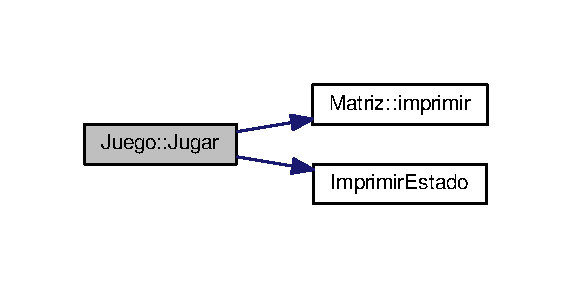
\includegraphics[width=274pt]{class_juego_a4a542c33876cbe1a1ea4706197fc6a17_cgraph}
\end{center}
\end{figure}




Here is the caller graph for this function\-:
\nopagebreak
\begin{figure}[H]
\begin{center}
\leavevmode
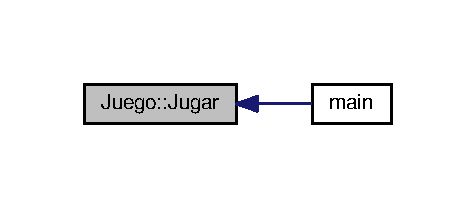
\includegraphics[width=228pt]{class_juego_a4a542c33876cbe1a1ea4706197fc6a17_icgraph}
\end{center}
\end{figure}




The documentation for this class was generated from the following files\-:\begin{DoxyCompactItemize}
\item 
{\bf Juego.\-h}\item 
{\bf Juego.\-cpp}\end{DoxyCompactItemize}

\section{Lobo Class Reference}
\label{class_lobo}\index{Lobo@{Lobo}}


{\ttfamily \#include $<$Lobo.\-h$>$}



Inheritance diagram for Lobo\-:
\nopagebreak
\begin{figure}[H]
\begin{center}
\leavevmode
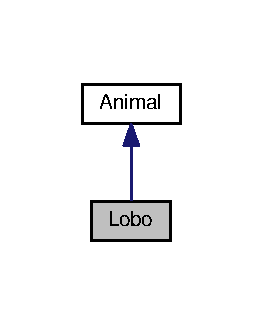
\includegraphics[width=126pt]{class_lobo__inherit__graph}
\end{center}
\end{figure}


Collaboration diagram for Lobo\-:
\nopagebreak
\begin{figure}[H]
\begin{center}
\leavevmode
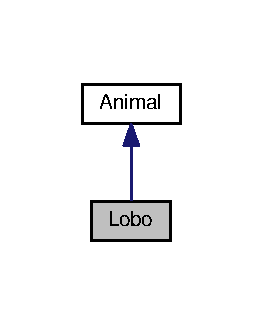
\includegraphics[width=126pt]{class_lobo__coll__graph}
\end{center}
\end{figure}
\subsection*{Public Member Functions}
\begin{DoxyCompactItemize}
\item 
{\bf Lobo} ()
\item 
virtual {\bf $\sim$\-Lobo} ()
\item 
void {\bf operator!} ()
\item 
void {\bf operator++} (int)
\item 
void {\bf operator$\sim$} ()
\item 
void {\bf operator-\/-\/} (int)
\item 
void {\bf macho\-Alfa} ()
\end{DoxyCompactItemize}
\subsection*{Additional Inherited Members}


\subsection{Constructor \& Destructor Documentation}
\index{Lobo@{Lobo}!Lobo@{Lobo}}
\index{Lobo@{Lobo}!Lobo@{Lobo}}
\subsubsection[{Lobo}]{\setlength{\rightskip}{0pt plus 5cm}Lobo\-::\-Lobo (
\begin{DoxyParamCaption}
{}
\end{DoxyParamCaption}
)}\label{class_lobo_a5c6b593887d794ea47abcc7af82a4090}


Here is the caller graph for this function\-:
\nopagebreak
\begin{figure}[H]
\begin{center}
\leavevmode
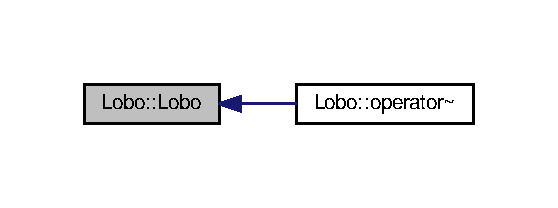
\includegraphics[width=268pt]{class_lobo_a5c6b593887d794ea47abcc7af82a4090_icgraph}
\end{center}
\end{figure}


\index{Lobo@{Lobo}!$\sim$\-Lobo@{$\sim$\-Lobo}}
\index{$\sim$\-Lobo@{$\sim$\-Lobo}!Lobo@{Lobo}}
\subsubsection[{$\sim$\-Lobo}]{\setlength{\rightskip}{0pt plus 5cm}Lobo\-::$\sim$\-Lobo (
\begin{DoxyParamCaption}
{}
\end{DoxyParamCaption}
)\hspace{0.3cm}{\ttfamily [virtual]}}\label{class_lobo_ac3f55f7ba044fc5a20fbcbeed644ce54}


\subsection{Member Function Documentation}
\index{Lobo@{Lobo}!macho\-Alfa@{macho\-Alfa}}
\index{macho\-Alfa@{macho\-Alfa}!Lobo@{Lobo}}
\subsubsection[{macho\-Alfa}]{\setlength{\rightskip}{0pt plus 5cm}void Lobo\-::macho\-Alfa (
\begin{DoxyParamCaption}
{}
\end{DoxyParamCaption}
)\hspace{0.3cm}{\ttfamily [virtual]}}\label{class_lobo_a50dac66859d049bc94d0d741297bae3c}


Implements {\bf Animal} \doxyref{}{p.}{class_animal_af0195b0b3cec650e1ece60edd6e031ef}.



Here is the call graph for this function\-:
\nopagebreak
\begin{figure}[H]
\begin{center}
\leavevmode
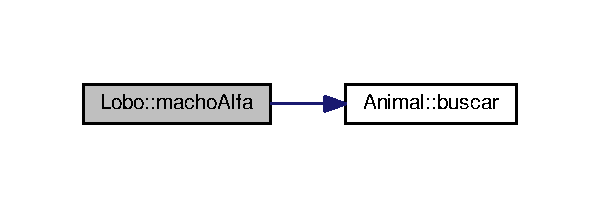
\includegraphics[width=288pt]{class_lobo_a50dac66859d049bc94d0d741297bae3c_cgraph}
\end{center}
\end{figure}


\index{Lobo@{Lobo}!operator!@{operator!}}
\index{operator!@{operator!}!Lobo@{Lobo}}
\subsubsection[{operator!}]{\setlength{\rightskip}{0pt plus 5cm}void Lobo\-::operator! (
\begin{DoxyParamCaption}
{}
\end{DoxyParamCaption}
)\hspace{0.3cm}{\ttfamily [virtual]}}\label{class_lobo_a3d93cb16a5a0f1e93e0321116227ac14}


Implements {\bf Animal} \doxyref{}{p.}{class_animal_a0def749264daf97160df081b0c028ffe}.



Here is the call graph for this function\-:
\nopagebreak
\begin{figure}[H]
\begin{center}
\leavevmode
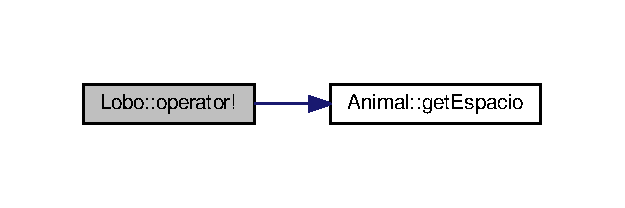
\includegraphics[width=300pt]{class_lobo_a3d93cb16a5a0f1e93e0321116227ac14_cgraph}
\end{center}
\end{figure}


\index{Lobo@{Lobo}!operator++@{operator++}}
\index{operator++@{operator++}!Lobo@{Lobo}}
\subsubsection[{operator++}]{\setlength{\rightskip}{0pt plus 5cm}void Lobo\-::operator++ (
\begin{DoxyParamCaption}
\item[{int}]{}
\end{DoxyParamCaption}
)\hspace{0.3cm}{\ttfamily [virtual]}}\label{class_lobo_a49fcb341d6af488987d7c8a10ad45b38}


Implements {\bf Animal} \doxyref{}{p.}{class_animal_a82bc2c40b773a232548f961053f9067d}.



Here is the call graph for this function\-:
\nopagebreak
\begin{figure}[H]
\begin{center}
\leavevmode
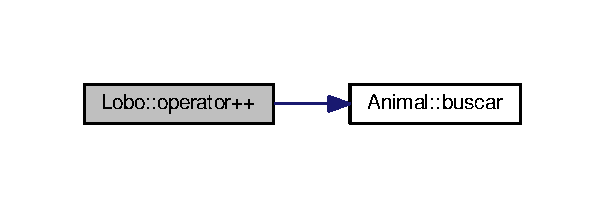
\includegraphics[width=290pt]{class_lobo_a49fcb341d6af488987d7c8a10ad45b38_cgraph}
\end{center}
\end{figure}


\index{Lobo@{Lobo}!operator-\/-\/@{operator-\/-\/}}
\index{operator-\/-\/@{operator-\/-\/}!Lobo@{Lobo}}
\subsubsection[{operator-\/-\/}]{\setlength{\rightskip}{0pt plus 5cm}void Lobo\-::operator-\/-\/ (
\begin{DoxyParamCaption}
\item[{int}]{}
\end{DoxyParamCaption}
)\hspace{0.3cm}{\ttfamily [virtual]}}\label{class_lobo_a880e124e43304deac3aa16188ed7fec6}


Implements {\bf Animal} \doxyref{}{p.}{class_animal_a43d005a7b5dfa9888a9db21e1e864609}.

\index{Lobo@{Lobo}!operator$\sim$@{operator$\sim$}}
\index{operator$\sim$@{operator$\sim$}!Lobo@{Lobo}}
\subsubsection[{operator$\sim$}]{\setlength{\rightskip}{0pt plus 5cm}void Lobo\-::operator$\sim$ (
\begin{DoxyParamCaption}
{}
\end{DoxyParamCaption}
)\hspace{0.3cm}{\ttfamily [virtual]}}\label{class_lobo_a2b4bba4b6d6efa24af4d8e3b986dc7f2}


Implements {\bf Animal} \doxyref{}{p.}{class_animal_a6539ec18d8975982b65de76d8e5638f0}.



Here is the call graph for this function\-:
\nopagebreak
\begin{figure}[H]
\begin{center}
\leavevmode
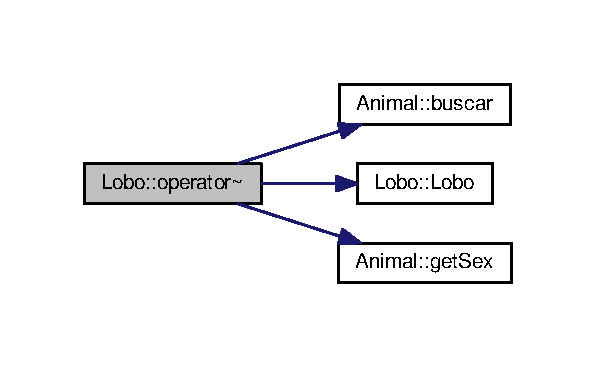
\includegraphics[width=286pt]{class_lobo_a2b4bba4b6d6efa24af4d8e3b986dc7f2_cgraph}
\end{center}
\end{figure}




The documentation for this class was generated from the following files\-:\begin{DoxyCompactItemize}
\item 
{\bf Lobo.\-h}\item 
{\bf Lobo.\-cpp}\end{DoxyCompactItemize}

\section{Matriz Class Reference}
\label{class_matriz}\index{Matriz@{Matriz}}


{\ttfamily \#include $<$Matriz.\-h$>$}



Collaboration diagram for Matriz\-:
\nopagebreak
\begin{figure}[H]
\begin{center}
\leavevmode
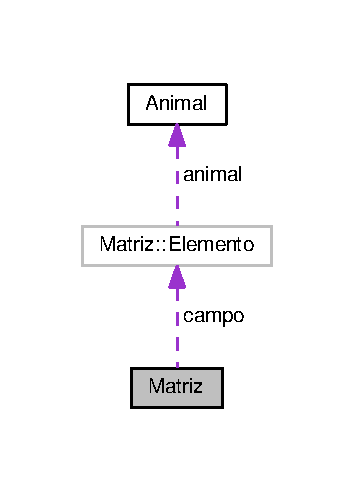
\includegraphics[width=170pt]{class_matriz__coll__graph}
\end{center}
\end{figure}
\subsection*{Public Member Functions}
\begin{DoxyCompactItemize}
\item 
{\bf Matriz} (string text)
\item 
virtual {\bf $\sim$\-Matriz} ()
\item 
void {\bf imprimir} ()
\end{DoxyCompactItemize}
\subsection*{Static Public Attributes}
\begin{DoxyCompactItemize}
\item 
static int {\bf numfilas} = 0
\item 
static int {\bf numcolumnas} = 0
\item 
static Elemento $\ast$$\ast$ {\bf campo} = N\-U\-L\-L
\end{DoxyCompactItemize}


\subsection{Constructor \& Destructor Documentation}
\index{Matriz@{Matriz}!Matriz@{Matriz}}
\index{Matriz@{Matriz}!Matriz@{Matriz}}
\subsubsection[{Matriz}]{\setlength{\rightskip}{0pt plus 5cm}Matriz\-::\-Matriz (
\begin{DoxyParamCaption}
\item[{string}]{text}
\end{DoxyParamCaption}
)}\label{class_matriz_a40756c1bbe79a77fded36a7c23f678e7}
\index{Matriz@{Matriz}!$\sim$\-Matriz@{$\sim$\-Matriz}}
\index{$\sim$\-Matriz@{$\sim$\-Matriz}!Matriz@{Matriz}}
\subsubsection[{$\sim$\-Matriz}]{\setlength{\rightskip}{0pt plus 5cm}Matriz\-::$\sim$\-Matriz (
\begin{DoxyParamCaption}
{}
\end{DoxyParamCaption}
)\hspace{0.3cm}{\ttfamily [virtual]}}\label{class_matriz_a2092b7a289ecec369e1da407d5839f5a}


\subsection{Member Function Documentation}
\index{Matriz@{Matriz}!imprimir@{imprimir}}
\index{imprimir@{imprimir}!Matriz@{Matriz}}
\subsubsection[{imprimir}]{\setlength{\rightskip}{0pt plus 5cm}void Matriz\-::imprimir (
\begin{DoxyParamCaption}
{}
\end{DoxyParamCaption}
)}\label{class_matriz_af70054abb48b35fcf67e26ecaea43fde}


Here is the caller graph for this function\-:
\nopagebreak
\begin{figure}[H]
\begin{center}
\leavevmode
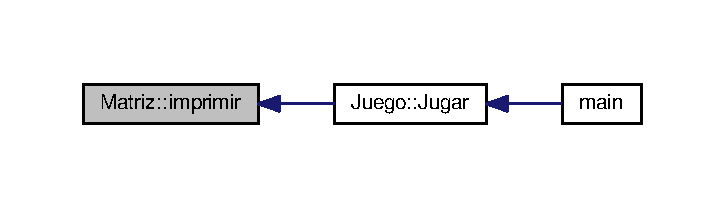
\includegraphics[width=348pt]{class_matriz_af70054abb48b35fcf67e26ecaea43fde_icgraph}
\end{center}
\end{figure}




\subsection{Member Data Documentation}
\index{Matriz@{Matriz}!campo@{campo}}
\index{campo@{campo}!Matriz@{Matriz}}
\subsubsection[{campo}]{\setlength{\rightskip}{0pt plus 5cm}Matriz\-::\-Elemento $\ast$$\ast$ Matriz\-::campo = N\-U\-L\-L\hspace{0.3cm}{\ttfamily [static]}}\label{class_matriz_a032ccdc0809d49523ffb99cba18d521e}
\index{Matriz@{Matriz}!numcolumnas@{numcolumnas}}
\index{numcolumnas@{numcolumnas}!Matriz@{Matriz}}
\subsubsection[{numcolumnas}]{\setlength{\rightskip}{0pt plus 5cm}int Matriz\-::numcolumnas = 0\hspace{0.3cm}{\ttfamily [static]}}\label{class_matriz_a3d97ee57664483d8ffce52aa9360d37b}
\index{Matriz@{Matriz}!numfilas@{numfilas}}
\index{numfilas@{numfilas}!Matriz@{Matriz}}
\subsubsection[{numfilas}]{\setlength{\rightskip}{0pt plus 5cm}int Matriz\-::numfilas = 0\hspace{0.3cm}{\ttfamily [static]}}\label{class_matriz_a2df02e4f2af8f0bf765e24d7bc9ca475}


The documentation for this class was generated from the following files\-:\begin{DoxyCompactItemize}
\item 
{\bf Matriz.\-h}\item 
{\bf Matriz.\-cpp}\end{DoxyCompactItemize}

\section{Oveja Class Reference}
\label{class_oveja}\index{Oveja@{Oveja}}


{\ttfamily \#include $<$Oveja.\-h$>$}



Inheritance diagram for Oveja\-:
\nopagebreak
\begin{figure}[H]
\begin{center}
\leavevmode
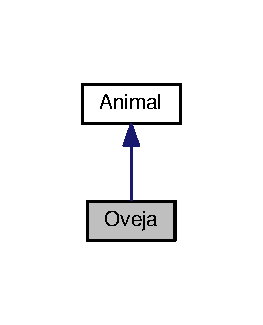
\includegraphics[width=126pt]{class_oveja__inherit__graph}
\end{center}
\end{figure}


Collaboration diagram for Oveja\-:
\nopagebreak
\begin{figure}[H]
\begin{center}
\leavevmode
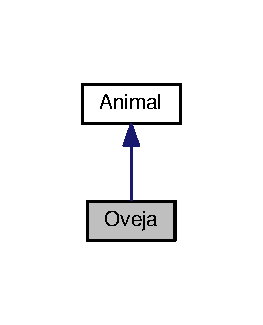
\includegraphics[width=126pt]{class_oveja__coll__graph}
\end{center}
\end{figure}
\subsection*{Public Member Functions}
\begin{DoxyCompactItemize}
\item 
{\bf Oveja} ()
\item 
virtual {\bf $\sim$\-Oveja} ()
\item 
void {\bf operator!} ()
\item 
void {\bf operator++} (int)
\item 
void {\bf operator$\sim$} ()
\item 
void {\bf operator-\/-\/} (int)
\item 
void {\bf macho\-Alfa} ()
\end{DoxyCompactItemize}
\subsection*{Additional Inherited Members}


\subsection{Constructor \& Destructor Documentation}
\index{Oveja@{Oveja}!Oveja@{Oveja}}
\index{Oveja@{Oveja}!Oveja@{Oveja}}
\subsubsection[{Oveja}]{\setlength{\rightskip}{0pt plus 5cm}Oveja\-::\-Oveja (
\begin{DoxyParamCaption}
{}
\end{DoxyParamCaption}
)}\label{class_oveja_a816d51452247a98f55372b7407de0366}


Here is the caller graph for this function\-:
\nopagebreak
\begin{figure}[H]
\begin{center}
\leavevmode
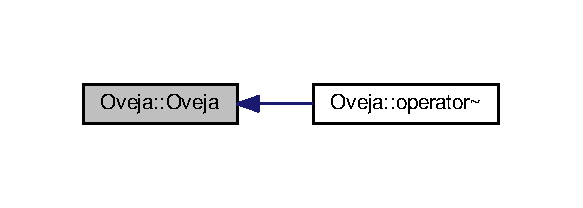
\includegraphics[width=280pt]{class_oveja_a816d51452247a98f55372b7407de0366_icgraph}
\end{center}
\end{figure}


\index{Oveja@{Oveja}!$\sim$\-Oveja@{$\sim$\-Oveja}}
\index{$\sim$\-Oveja@{$\sim$\-Oveja}!Oveja@{Oveja}}
\subsubsection[{$\sim$\-Oveja}]{\setlength{\rightskip}{0pt plus 5cm}Oveja\-::$\sim$\-Oveja (
\begin{DoxyParamCaption}
{}
\end{DoxyParamCaption}
)\hspace{0.3cm}{\ttfamily [virtual]}}\label{class_oveja_a90e76a79dba9138b13c26ba0b1b3c2cf}


\subsection{Member Function Documentation}
\index{Oveja@{Oveja}!macho\-Alfa@{macho\-Alfa}}
\index{macho\-Alfa@{macho\-Alfa}!Oveja@{Oveja}}
\subsubsection[{macho\-Alfa}]{\setlength{\rightskip}{0pt plus 5cm}void Oveja\-::macho\-Alfa (
\begin{DoxyParamCaption}
{}
\end{DoxyParamCaption}
)\hspace{0.3cm}{\ttfamily [virtual]}}\label{class_oveja_a7821f1605ff38842fac3d79d3ad534c6}


Implements {\bf Animal} \doxyref{}{p.}{class_animal_af0195b0b3cec650e1ece60edd6e031ef}.

\index{Oveja@{Oveja}!operator!@{operator!}}
\index{operator!@{operator!}!Oveja@{Oveja}}
\subsubsection[{operator!}]{\setlength{\rightskip}{0pt plus 5cm}void Oveja\-::operator! (
\begin{DoxyParamCaption}
{}
\end{DoxyParamCaption}
)\hspace{0.3cm}{\ttfamily [virtual]}}\label{class_oveja_ae63ca7bb074bf36591e3f12f2c7a9037}


Implements {\bf Animal} \doxyref{}{p.}{class_animal_a0def749264daf97160df081b0c028ffe}.



Here is the call graph for this function\-:
\nopagebreak
\begin{figure}[H]
\begin{center}
\leavevmode
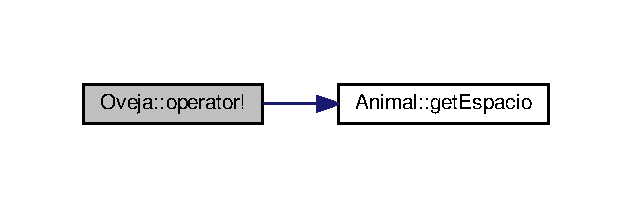
\includegraphics[width=304pt]{class_oveja_ae63ca7bb074bf36591e3f12f2c7a9037_cgraph}
\end{center}
\end{figure}


\index{Oveja@{Oveja}!operator++@{operator++}}
\index{operator++@{operator++}!Oveja@{Oveja}}
\subsubsection[{operator++}]{\setlength{\rightskip}{0pt plus 5cm}void Oveja\-::operator++ (
\begin{DoxyParamCaption}
\item[{int}]{}
\end{DoxyParamCaption}
)\hspace{0.3cm}{\ttfamily [virtual]}}\label{class_oveja_a80f81a1a32548bcec1e1b28ea5f9b503}


Implements {\bf Animal} \doxyref{}{p.}{class_animal_a82bc2c40b773a232548f961053f9067d}.

\index{Oveja@{Oveja}!operator-\/-\/@{operator-\/-\/}}
\index{operator-\/-\/@{operator-\/-\/}!Oveja@{Oveja}}
\subsubsection[{operator-\/-\/}]{\setlength{\rightskip}{0pt plus 5cm}void Oveja\-::operator-\/-\/ (
\begin{DoxyParamCaption}
\item[{int}]{}
\end{DoxyParamCaption}
)\hspace{0.3cm}{\ttfamily [virtual]}}\label{class_oveja_a3cc9887909aeb093a1133f48d6c13670}


Implements {\bf Animal} \doxyref{}{p.}{class_animal_a43d005a7b5dfa9888a9db21e1e864609}.

\index{Oveja@{Oveja}!operator$\sim$@{operator$\sim$}}
\index{operator$\sim$@{operator$\sim$}!Oveja@{Oveja}}
\subsubsection[{operator$\sim$}]{\setlength{\rightskip}{0pt plus 5cm}void Oveja\-::operator$\sim$ (
\begin{DoxyParamCaption}
{}
\end{DoxyParamCaption}
)\hspace{0.3cm}{\ttfamily [virtual]}}\label{class_oveja_a0ff5ac43f8a666b3b130de88da605fe2}


Implements {\bf Animal} \doxyref{}{p.}{class_animal_a6539ec18d8975982b65de76d8e5638f0}.



Here is the call graph for this function\-:
\nopagebreak
\begin{figure}[H]
\begin{center}
\leavevmode
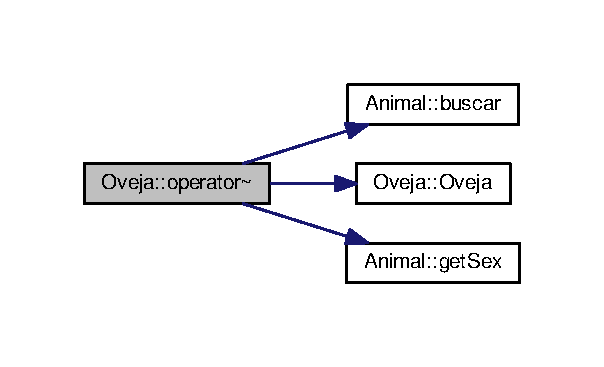
\includegraphics[width=290pt]{class_oveja_a0ff5ac43f8a666b3b130de88da605fe2_cgraph}
\end{center}
\end{figure}




The documentation for this class was generated from the following files\-:\begin{DoxyCompactItemize}
\item 
{\bf Oveja.\-h}\item 
{\bf Oveja.\-cpp}\end{DoxyCompactItemize}

\section{Raton Class Reference}
\label{class_raton}\index{Raton@{Raton}}


{\ttfamily \#include $<$Raton.\-h$>$}



Inheritance diagram for Raton\-:
\nopagebreak
\begin{figure}[H]
\begin{center}
\leavevmode
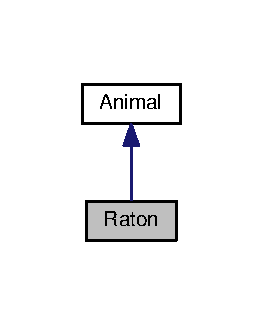
\includegraphics[width=126pt]{class_raton__inherit__graph}
\end{center}
\end{figure}


Collaboration diagram for Raton\-:
\nopagebreak
\begin{figure}[H]
\begin{center}
\leavevmode
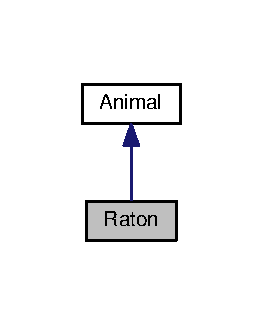
\includegraphics[width=126pt]{class_raton__coll__graph}
\end{center}
\end{figure}
\subsection*{Public Member Functions}
\begin{DoxyCompactItemize}
\item 
{\bf Raton} ()
\item 
virtual {\bf $\sim$\-Raton} ()
\item 
void {\bf operator!} ()
\item 
void {\bf operator++} (int)
\item 
void {\bf operator$\sim$} ()
\item 
void {\bf operator-\/-\/} (int)
\item 
void {\bf macho\-Alfa} ()
\end{DoxyCompactItemize}
\subsection*{Additional Inherited Members}


\subsection{Constructor \& Destructor Documentation}
\index{Raton@{Raton}!Raton@{Raton}}
\index{Raton@{Raton}!Raton@{Raton}}
\subsubsection[{Raton}]{\setlength{\rightskip}{0pt plus 5cm}Raton\-::\-Raton (
\begin{DoxyParamCaption}
{}
\end{DoxyParamCaption}
)}\label{class_raton_a9981955d139254e7a3990ebbf4d6d6d2}


Here is the caller graph for this function\-:
\nopagebreak
\begin{figure}[H]
\begin{center}
\leavevmode
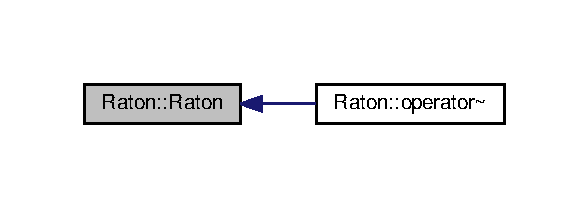
\includegraphics[width=282pt]{class_raton_a9981955d139254e7a3990ebbf4d6d6d2_icgraph}
\end{center}
\end{figure}


\index{Raton@{Raton}!$\sim$\-Raton@{$\sim$\-Raton}}
\index{$\sim$\-Raton@{$\sim$\-Raton}!Raton@{Raton}}
\subsubsection[{$\sim$\-Raton}]{\setlength{\rightskip}{0pt plus 5cm}Raton\-::$\sim$\-Raton (
\begin{DoxyParamCaption}
{}
\end{DoxyParamCaption}
)\hspace{0.3cm}{\ttfamily [virtual]}}\label{class_raton_a65e9e02f328adbda8d588548a3b1d76b}


\subsection{Member Function Documentation}
\index{Raton@{Raton}!macho\-Alfa@{macho\-Alfa}}
\index{macho\-Alfa@{macho\-Alfa}!Raton@{Raton}}
\subsubsection[{macho\-Alfa}]{\setlength{\rightskip}{0pt plus 5cm}void Raton\-::macho\-Alfa (
\begin{DoxyParamCaption}
{}
\end{DoxyParamCaption}
)\hspace{0.3cm}{\ttfamily [virtual]}}\label{class_raton_a6b74bd921ef203b600be27e9c28a14c8}


Implements {\bf Animal} \doxyref{}{p.}{class_animal_af0195b0b3cec650e1ece60edd6e031ef}.

\index{Raton@{Raton}!operator!@{operator!}}
\index{operator!@{operator!}!Raton@{Raton}}
\subsubsection[{operator!}]{\setlength{\rightskip}{0pt plus 5cm}void Raton\-::operator! (
\begin{DoxyParamCaption}
{}
\end{DoxyParamCaption}
)\hspace{0.3cm}{\ttfamily [virtual]}}\label{class_raton_a7d07f8b6493b3ee9130ba0143acd755f}


Implements {\bf Animal} \doxyref{}{p.}{class_animal_a0def749264daf97160df081b0c028ffe}.



Here is the call graph for this function\-:
\nopagebreak
\begin{figure}[H]
\begin{center}
\leavevmode
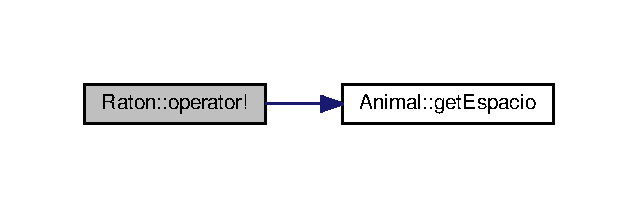
\includegraphics[width=306pt]{class_raton_a7d07f8b6493b3ee9130ba0143acd755f_cgraph}
\end{center}
\end{figure}


\index{Raton@{Raton}!operator++@{operator++}}
\index{operator++@{operator++}!Raton@{Raton}}
\subsubsection[{operator++}]{\setlength{\rightskip}{0pt plus 5cm}void Raton\-::operator++ (
\begin{DoxyParamCaption}
\item[{int}]{}
\end{DoxyParamCaption}
)\hspace{0.3cm}{\ttfamily [virtual]}}\label{class_raton_acd6d6d7e944c9212e368dab9ffb32b72}


Implements {\bf Animal} \doxyref{}{p.}{class_animal_a82bc2c40b773a232548f961053f9067d}.

\index{Raton@{Raton}!operator-\/-\/@{operator-\/-\/}}
\index{operator-\/-\/@{operator-\/-\/}!Raton@{Raton}}
\subsubsection[{operator-\/-\/}]{\setlength{\rightskip}{0pt plus 5cm}void Raton\-::operator-\/-\/ (
\begin{DoxyParamCaption}
\item[{int}]{}
\end{DoxyParamCaption}
)\hspace{0.3cm}{\ttfamily [virtual]}}\label{class_raton_ac6c595aae5f66043f2e3cce1dd38e0e0}


Implements {\bf Animal} \doxyref{}{p.}{class_animal_a43d005a7b5dfa9888a9db21e1e864609}.

\index{Raton@{Raton}!operator$\sim$@{operator$\sim$}}
\index{operator$\sim$@{operator$\sim$}!Raton@{Raton}}
\subsubsection[{operator$\sim$}]{\setlength{\rightskip}{0pt plus 5cm}void Raton\-::operator$\sim$ (
\begin{DoxyParamCaption}
{}
\end{DoxyParamCaption}
)\hspace{0.3cm}{\ttfamily [virtual]}}\label{class_raton_a7ec71ea95a98d13bf2cccf108b3c76d6}


Implements {\bf Animal} \doxyref{}{p.}{class_animal_a6539ec18d8975982b65de76d8e5638f0}.



Here is the call graph for this function\-:
\nopagebreak
\begin{figure}[H]
\begin{center}
\leavevmode
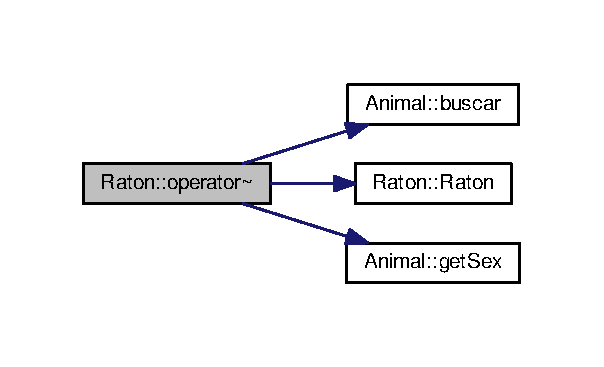
\includegraphics[width=290pt]{class_raton_a7ec71ea95a98d13bf2cccf108b3c76d6_cgraph}
\end{center}
\end{figure}




The documentation for this class was generated from the following files\-:\begin{DoxyCompactItemize}
\item 
{\bf Raton.\-h}\item 
{\bf Raton.\-cpp}\end{DoxyCompactItemize}

\section{Zorro Class Reference}
\label{class_zorro}\index{Zorro@{Zorro}}


{\ttfamily \#include $<$Zorro.\-h$>$}



Inheritance diagram for Zorro\-:
\nopagebreak
\begin{figure}[H]
\begin{center}
\leavevmode
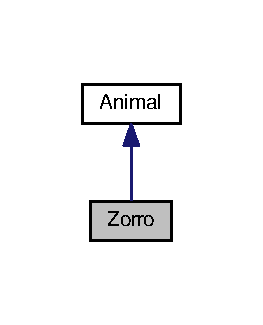
\includegraphics[width=126pt]{class_zorro__inherit__graph}
\end{center}
\end{figure}


Collaboration diagram for Zorro\-:
\nopagebreak
\begin{figure}[H]
\begin{center}
\leavevmode
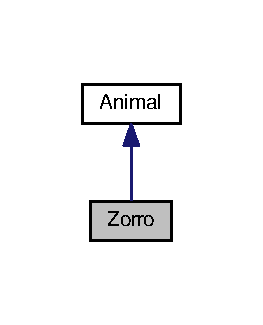
\includegraphics[width=126pt]{class_zorro__coll__graph}
\end{center}
\end{figure}
\subsection*{Public Member Functions}
\begin{DoxyCompactItemize}
\item 
{\bf Zorro} ()
\item 
virtual {\bf $\sim$\-Zorro} ()
\item 
void {\bf operator!} ()
\item 
void {\bf operator++} (int)
\item 
void {\bf operator$\sim$} ()
\item 
void {\bf operator-\/-\/} (int)
\item 
void {\bf macho\-Alfa} ()
\end{DoxyCompactItemize}
\subsection*{Additional Inherited Members}


\subsection{Constructor \& Destructor Documentation}
\index{Zorro@{Zorro}!Zorro@{Zorro}}
\index{Zorro@{Zorro}!Zorro@{Zorro}}
\subsubsection[{Zorro}]{\setlength{\rightskip}{0pt plus 5cm}Zorro\-::\-Zorro (
\begin{DoxyParamCaption}
{}
\end{DoxyParamCaption}
)}\label{class_zorro_adb6072a36faa243b1c185ec3e566f556}


Here is the caller graph for this function\-:
\nopagebreak
\begin{figure}[H]
\begin{center}
\leavevmode
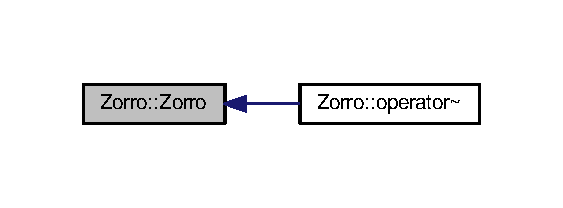
\includegraphics[width=270pt]{class_zorro_adb6072a36faa243b1c185ec3e566f556_icgraph}
\end{center}
\end{figure}


\index{Zorro@{Zorro}!$\sim$\-Zorro@{$\sim$\-Zorro}}
\index{$\sim$\-Zorro@{$\sim$\-Zorro}!Zorro@{Zorro}}
\subsubsection[{$\sim$\-Zorro}]{\setlength{\rightskip}{0pt plus 5cm}Zorro\-::$\sim$\-Zorro (
\begin{DoxyParamCaption}
{}
\end{DoxyParamCaption}
)\hspace{0.3cm}{\ttfamily [virtual]}}\label{class_zorro_a73fe75fd4746a9347da559ffaa741842}


\subsection{Member Function Documentation}
\index{Zorro@{Zorro}!macho\-Alfa@{macho\-Alfa}}
\index{macho\-Alfa@{macho\-Alfa}!Zorro@{Zorro}}
\subsubsection[{macho\-Alfa}]{\setlength{\rightskip}{0pt plus 5cm}void Zorro\-::macho\-Alfa (
\begin{DoxyParamCaption}
{}
\end{DoxyParamCaption}
)\hspace{0.3cm}{\ttfamily [virtual]}}\label{class_zorro_af1ca7e321452975225376d77905b4a5b}


Implements {\bf Animal} \doxyref{}{p.}{class_animal_af0195b0b3cec650e1ece60edd6e031ef}.

\index{Zorro@{Zorro}!operator!@{operator!}}
\index{operator!@{operator!}!Zorro@{Zorro}}
\subsubsection[{operator!}]{\setlength{\rightskip}{0pt plus 5cm}void Zorro\-::operator! (
\begin{DoxyParamCaption}
{}
\end{DoxyParamCaption}
)\hspace{0.3cm}{\ttfamily [virtual]}}\label{class_zorro_ab9ddecca664da566680332b0aa0ba225}


Implements {\bf Animal} \doxyref{}{p.}{class_animal_a0def749264daf97160df081b0c028ffe}.



Here is the call graph for this function\-:
\nopagebreak
\begin{figure}[H]
\begin{center}
\leavevmode
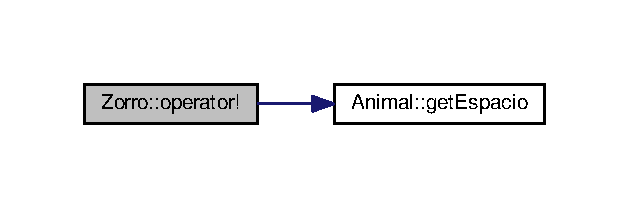
\includegraphics[width=302pt]{class_zorro_ab9ddecca664da566680332b0aa0ba225_cgraph}
\end{center}
\end{figure}


\index{Zorro@{Zorro}!operator++@{operator++}}
\index{operator++@{operator++}!Zorro@{Zorro}}
\subsubsection[{operator++}]{\setlength{\rightskip}{0pt plus 5cm}void Zorro\-::operator++ (
\begin{DoxyParamCaption}
\item[{int}]{}
\end{DoxyParamCaption}
)\hspace{0.3cm}{\ttfamily [virtual]}}\label{class_zorro_a747bf931fd26445891eb3af3785a0356}


Implements {\bf Animal} \doxyref{}{p.}{class_animal_a82bc2c40b773a232548f961053f9067d}.



Here is the call graph for this function\-:
\nopagebreak
\begin{figure}[H]
\begin{center}
\leavevmode
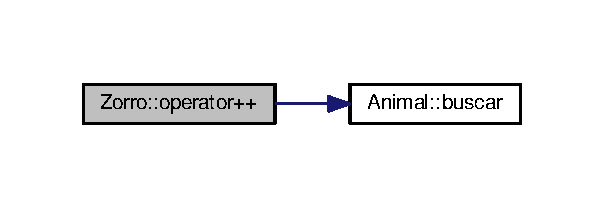
\includegraphics[width=290pt]{class_zorro_a747bf931fd26445891eb3af3785a0356_cgraph}
\end{center}
\end{figure}


\index{Zorro@{Zorro}!operator-\/-\/@{operator-\/-\/}}
\index{operator-\/-\/@{operator-\/-\/}!Zorro@{Zorro}}
\subsubsection[{operator-\/-\/}]{\setlength{\rightskip}{0pt plus 5cm}void Zorro\-::operator-\/-\/ (
\begin{DoxyParamCaption}
\item[{int}]{}
\end{DoxyParamCaption}
)\hspace{0.3cm}{\ttfamily [virtual]}}\label{class_zorro_ac6abad94a814d37f66f6a7698c75493e}


Implements {\bf Animal} \doxyref{}{p.}{class_animal_a43d005a7b5dfa9888a9db21e1e864609}.

\index{Zorro@{Zorro}!operator$\sim$@{operator$\sim$}}
\index{operator$\sim$@{operator$\sim$}!Zorro@{Zorro}}
\subsubsection[{operator$\sim$}]{\setlength{\rightskip}{0pt plus 5cm}void Zorro\-::operator$\sim$ (
\begin{DoxyParamCaption}
{}
\end{DoxyParamCaption}
)\hspace{0.3cm}{\ttfamily [virtual]}}\label{class_zorro_a9fdef26a109d506ac85b739c9920cc85}


Implements {\bf Animal} \doxyref{}{p.}{class_animal_a6539ec18d8975982b65de76d8e5638f0}.



Here is the call graph for this function\-:
\nopagebreak
\begin{figure}[H]
\begin{center}
\leavevmode
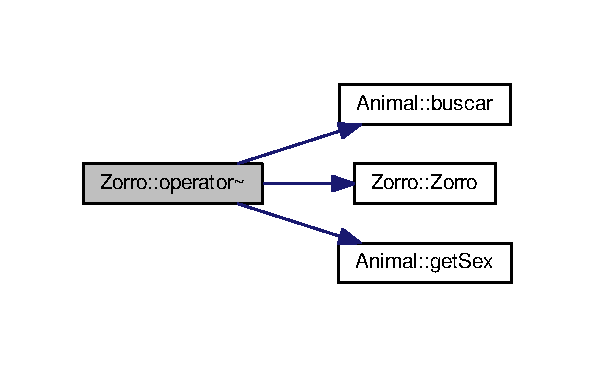
\includegraphics[width=286pt]{class_zorro_a9fdef26a109d506ac85b739c9920cc85_cgraph}
\end{center}
\end{figure}




The documentation for this class was generated from the following files\-:\begin{DoxyCompactItemize}
\item 
{\bf Zorro.\-h}\item 
{\bf Zorro.\-cpp}\end{DoxyCompactItemize}

\chapter{File Documentation}
\section{.dep.\-inc File Reference}
\label{_8dep_8inc}\index{.\-dep.\-inc@{.\-dep.\-inc}}

\section{Animal.\-cpp File Reference}
\label{_animal_8cpp}\index{Animal.\-cpp@{Animal.\-cpp}}
{\ttfamily \#include \char`\"{}Animal.\-h\char`\"{}}\\*
{\ttfamily \#include \char`\"{}Matriz.\-h\char`\"{}}\\*
Include dependency graph for Animal.\-cpp\-:
\nopagebreak
\begin{figure}[H]
\begin{center}
\leavevmode
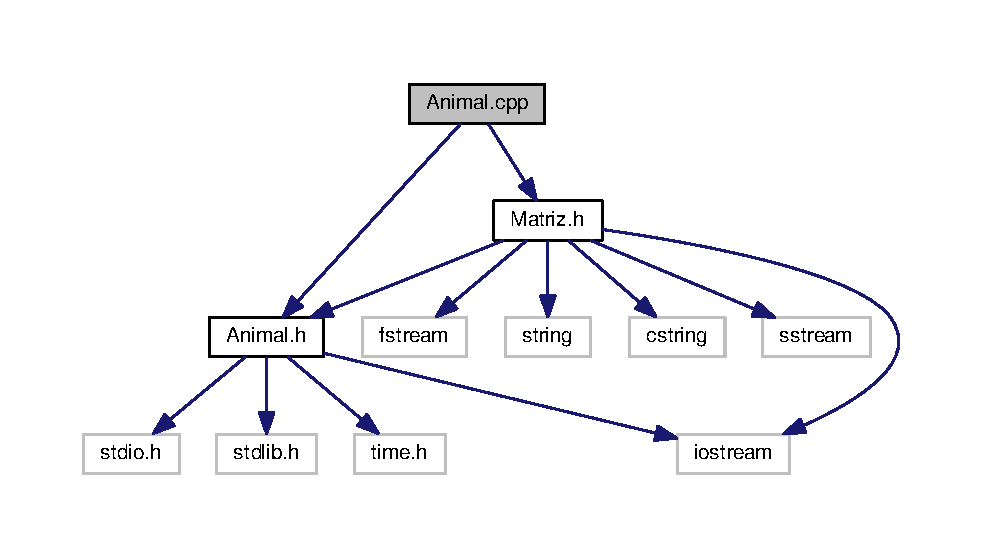
\includegraphics[width=350pt]{_animal_8cpp__incl}
\end{center}
\end{figure}

\section{Animal.\-h File Reference}
\label{_animal_8h}\index{Animal.\-h@{Animal.\-h}}
{\ttfamily \#include $<$iostream$>$}\\*
{\ttfamily \#include $<$stdio.\-h$>$}\\*
{\ttfamily \#include $<$stdlib.\-h$>$}\\*
{\ttfamily \#include $<$time.\-h$>$}\\*
Include dependency graph for Animal.\-h\-:
\nopagebreak
\begin{figure}[H]
\begin{center}
\leavevmode
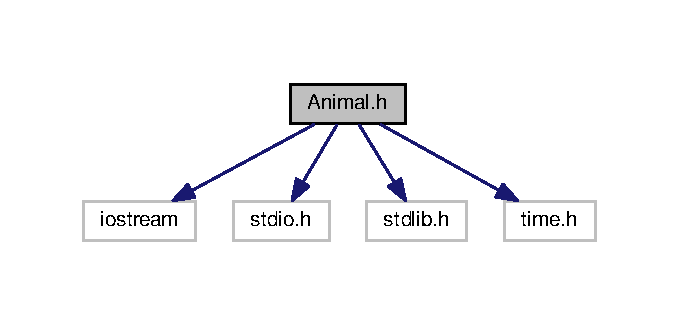
\includegraphics[width=326pt]{_animal_8h__incl}
\end{center}
\end{figure}
This graph shows which files directly or indirectly include this file\-:
\nopagebreak
\begin{figure}[H]
\begin{center}
\leavevmode
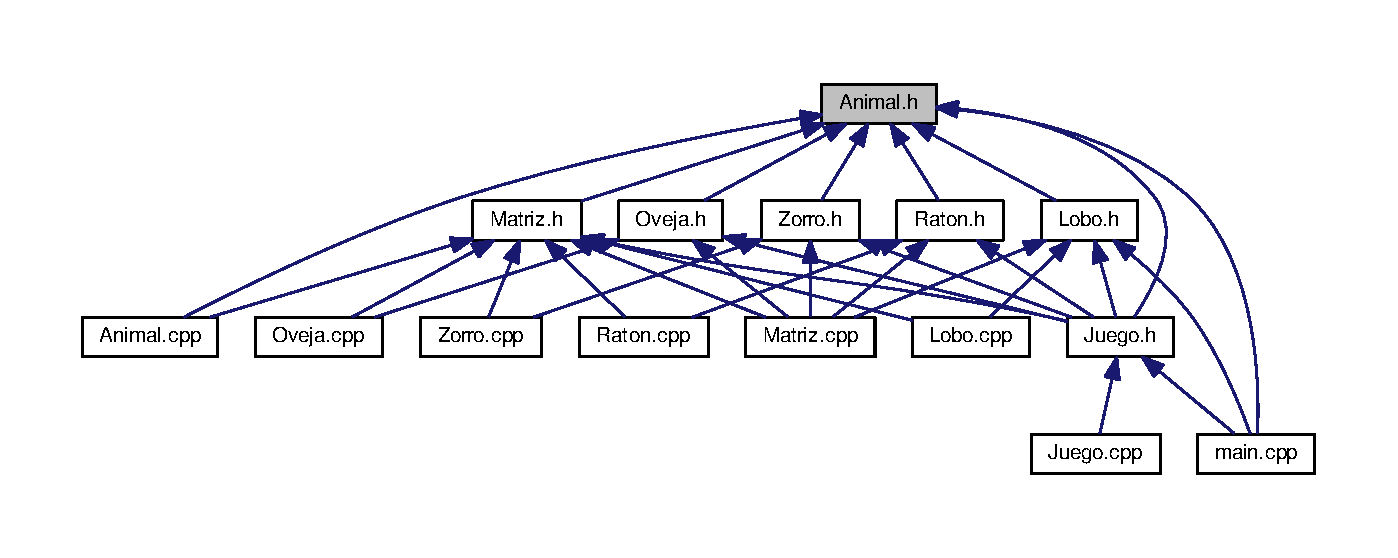
\includegraphics[width=350pt]{_animal_8h__dep__incl}
\end{center}
\end{figure}
\subsection*{Classes}
\begin{DoxyCompactItemize}
\item 
class {\bf Animal}
\end{DoxyCompactItemize}

\section{Juego.\-cpp File Reference}
\label{_juego_8cpp}\index{Juego.\-cpp@{Juego.\-cpp}}
{\ttfamily \#include \char`\"{}Juego.\-h\char`\"{}}\\*
Include dependency graph for Juego.\-cpp\-:
\nopagebreak
\begin{figure}[H]
\begin{center}
\leavevmode
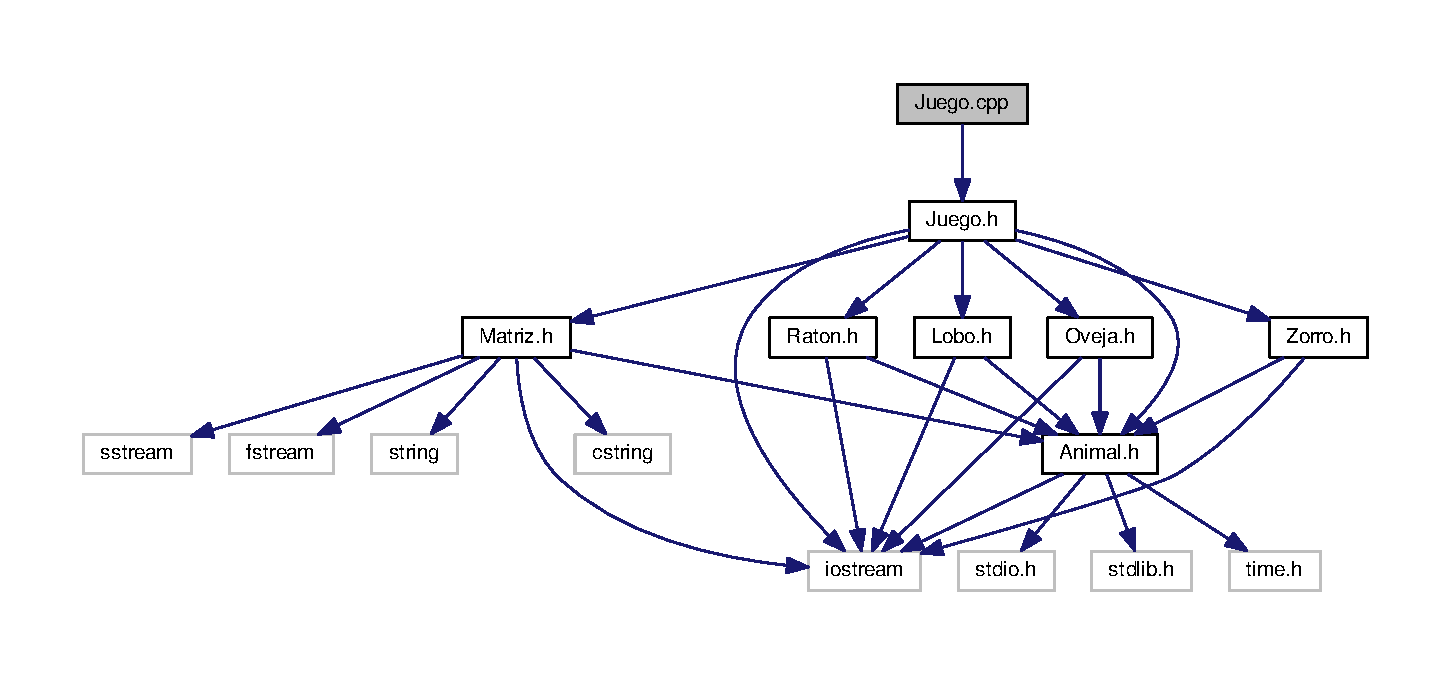
\includegraphics[width=350pt]{_juego_8cpp__incl}
\end{center}
\end{figure}
\subsection*{Functions}
\begin{DoxyCompactItemize}
\item 
{\footnotesize template$<$typename Any $>$ }\\void {\bf Imprimir\-Estado} (Any elemento)
\end{DoxyCompactItemize}


\subsection{Function Documentation}
\index{Juego.\-cpp@{Juego.\-cpp}!Imprimir\-Estado@{Imprimir\-Estado}}
\index{Imprimir\-Estado@{Imprimir\-Estado}!Juego.cpp@{Juego.\-cpp}}
\subsubsection[{Imprimir\-Estado}]{\setlength{\rightskip}{0pt plus 5cm}template$<$typename Any $>$ void Imprimir\-Estado (
\begin{DoxyParamCaption}
\item[{Any}]{elemento}
\end{DoxyParamCaption}
)}\label{_juego_8cpp_aa53a3e66a2fd096a2e10c3094ac41e70}


Here is the caller graph for this function\-:
\nopagebreak
\begin{figure}[H]
\begin{center}
\leavevmode
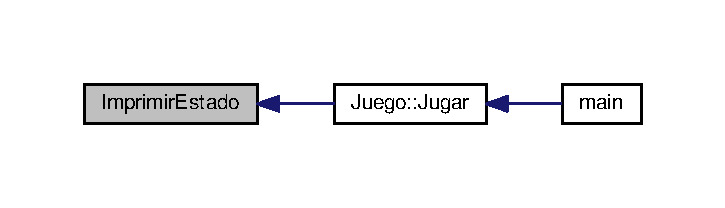
\includegraphics[width=348pt]{_juego_8cpp_aa53a3e66a2fd096a2e10c3094ac41e70_icgraph}
\end{center}
\end{figure}



\section{Juego.\-h File Reference}
\label{_juego_8h}\index{Juego.\-h@{Juego.\-h}}
{\ttfamily \#include \char`\"{}Matriz.\-h\char`\"{}}\\*
{\ttfamily \#include \char`\"{}Animal.\-h\char`\"{}}\\*
{\ttfamily \#include \char`\"{}Lobo.\-h\char`\"{}}\\*
{\ttfamily \#include \char`\"{}Oveja.\-h\char`\"{}}\\*
{\ttfamily \#include \char`\"{}Zorro.\-h\char`\"{}}\\*
{\ttfamily \#include \char`\"{}Raton.\-h\char`\"{}}\\*
{\ttfamily \#include $<$iostream$>$}\\*
Include dependency graph for Juego.\-h\-:
\nopagebreak
\begin{figure}[H]
\begin{center}
\leavevmode
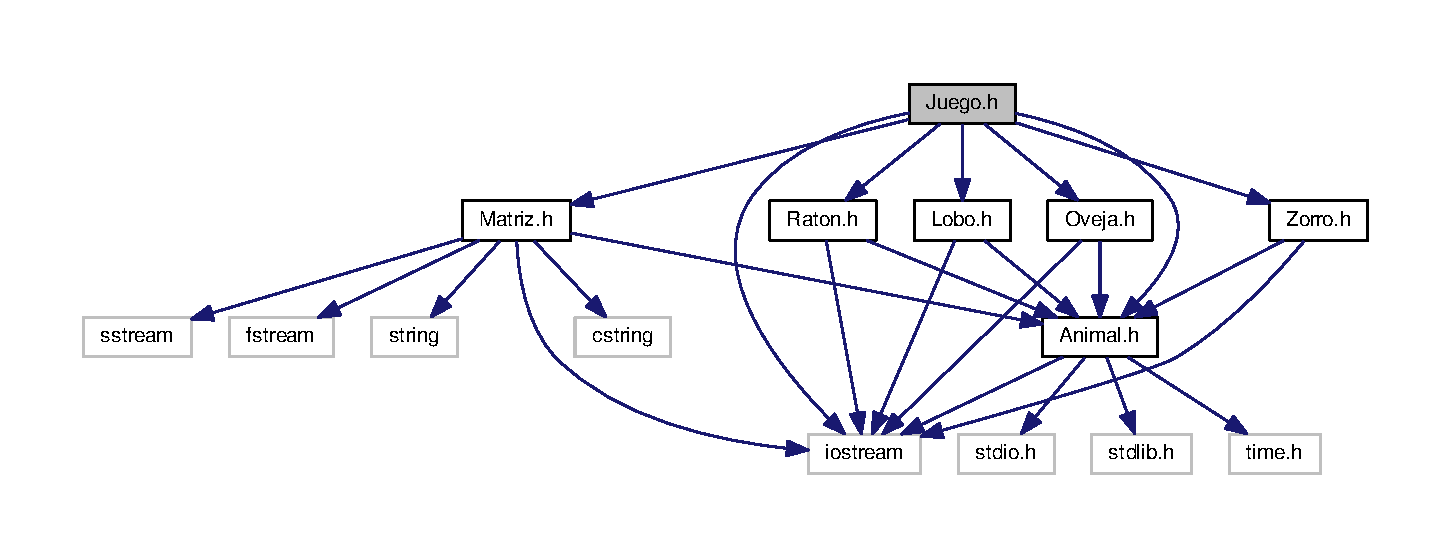
\includegraphics[width=350pt]{_juego_8h__incl}
\end{center}
\end{figure}
This graph shows which files directly or indirectly include this file\-:
\nopagebreak
\begin{figure}[H]
\begin{center}
\leavevmode
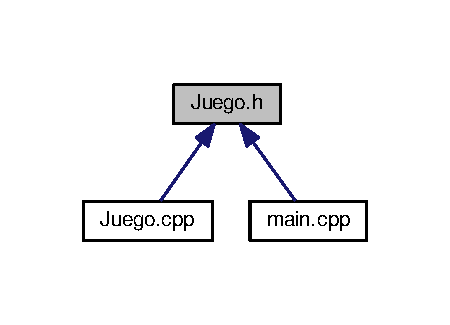
\includegraphics[width=216pt]{_juego_8h__dep__incl}
\end{center}
\end{figure}
\subsection*{Classes}
\begin{DoxyCompactItemize}
\item 
class {\bf Juego}
\end{DoxyCompactItemize}

\section{Lobo.\-cpp File Reference}
\label{_lobo_8cpp}\index{Lobo.\-cpp@{Lobo.\-cpp}}
{\ttfamily \#include \char`\"{}Lobo.\-h\char`\"{}}\\*
{\ttfamily \#include \char`\"{}Matriz.\-h\char`\"{}}\\*
Include dependency graph for Lobo.\-cpp\-:
\nopagebreak
\begin{figure}[H]
\begin{center}
\leavevmode
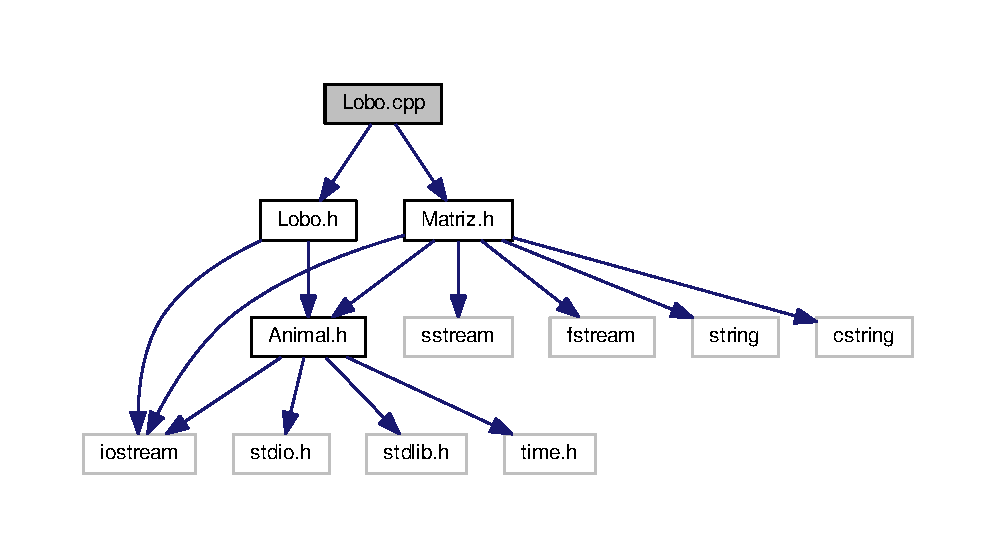
\includegraphics[width=350pt]{_lobo_8cpp__incl}
\end{center}
\end{figure}
\subsection*{Variables}
\begin{DoxyCompactItemize}
\item 
int {\bf opcion} =0
\end{DoxyCompactItemize}


\subsection{Variable Documentation}
\index{Lobo.\-cpp@{Lobo.\-cpp}!opcion@{opcion}}
\index{opcion@{opcion}!Lobo.cpp@{Lobo.\-cpp}}
\subsubsection[{opcion}]{\setlength{\rightskip}{0pt plus 5cm}int opcion =0}\label{_lobo_8cpp_a39f485a4773f634607a5caf635218a32}

\section{Lobo.\-h File Reference}
\label{_lobo_8h}\index{Lobo.\-h@{Lobo.\-h}}
{\ttfamily \#include $<$iostream$>$}\\*
{\ttfamily \#include \char`\"{}Animal.\-h\char`\"{}}\\*
Include dependency graph for Lobo.\-h\-:
\nopagebreak
\begin{figure}[H]
\begin{center}
\leavevmode
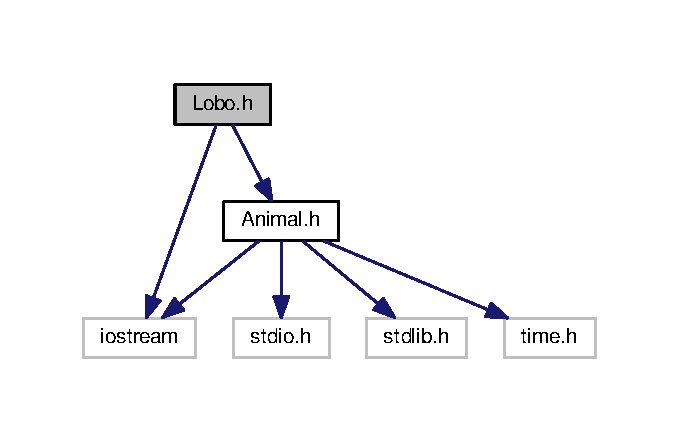
\includegraphics[width=326pt]{_lobo_8h__incl}
\end{center}
\end{figure}
This graph shows which files directly or indirectly include this file\-:
\nopagebreak
\begin{figure}[H]
\begin{center}
\leavevmode
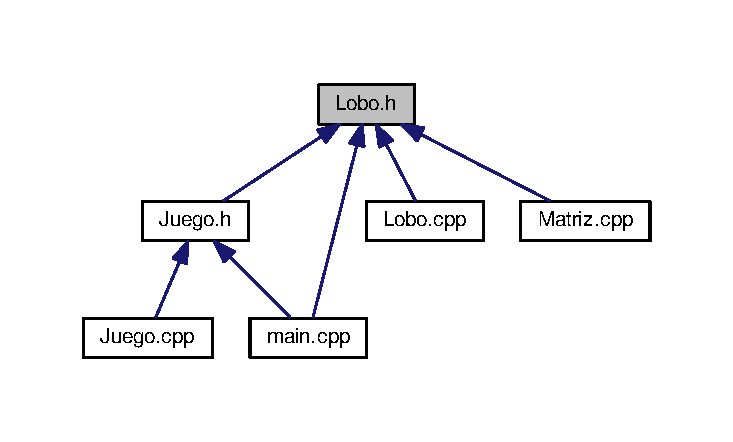
\includegraphics[width=350pt]{_lobo_8h__dep__incl}
\end{center}
\end{figure}
\subsection*{Classes}
\begin{DoxyCompactItemize}
\item 
class {\bf Lobo}
\end{DoxyCompactItemize}

\section{Referencia del Archivo main.\-cpp}
\label{main_8cpp}\index{main.\-cpp@{main.\-cpp}}
{\ttfamily \#include $<$iostream$>$}\\*
{\ttfamily \#include \char`\"{}List\-With\-Array.\-h\char`\"{}}\\*
{\ttfamily \#include \char`\"{}List\-With\-Pointer.\-h\char`\"{}}\\*
{\ttfamily \#include \char`\"{}Cell.\-h\char`\"{}}\\*
{\ttfamily \#include \char`\"{}Queue.\-h\char`\"{}}\\*
{\ttfamily \#include \char`\"{}Stack.\-h\char`\"{}}\\*
Dependencia gráfica adjunta para main.\-cpp\-:\nopagebreak
\begin{figure}[H]
\begin{center}
\leavevmode
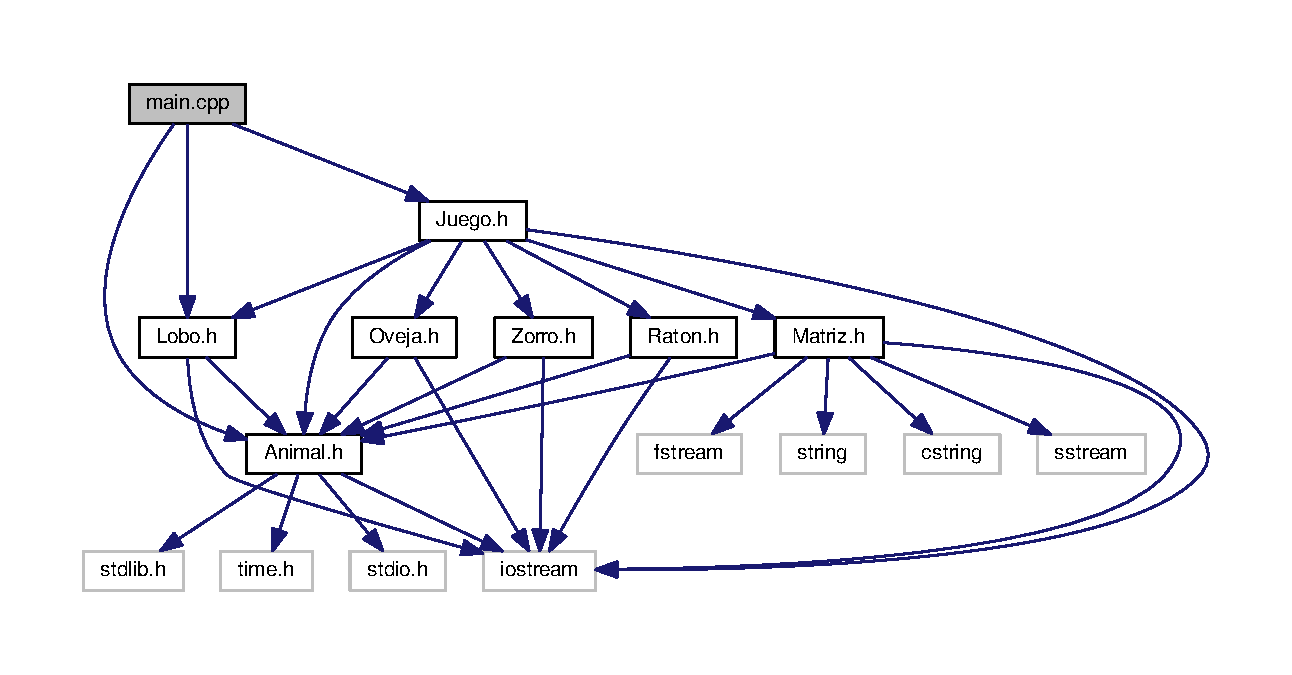
\includegraphics[width=350pt]{main_8cpp__incl}
\end{center}
\end{figure}
\subsection*{Funciones}
\begin{DoxyCompactItemize}
\item 
int {\bf main} (int argc, char $\ast$$\ast$argv)
\end{DoxyCompactItemize}


\subsection{Documentación de las funciones}
\index{main.\-cpp@{main.\-cpp}!main@{main}}
\index{main@{main}!main.cpp@{main.\-cpp}}
\subsubsection[{main}]{\setlength{\rightskip}{0pt plus 5cm}int main (
\begin{DoxyParamCaption}
\item[{int}]{argc, }
\item[{char $\ast$$\ast$}]{argv}
\end{DoxyParamCaption}
)}\label{main_8cpp_a3c04138a5bfe5d72780bb7e82a18e627}


Definición en la línea 9 del archivo main.\-cpp.



Gráfico de llamadas para esta función\-:\nopagebreak
\begin{figure}[H]
\begin{center}
\leavevmode
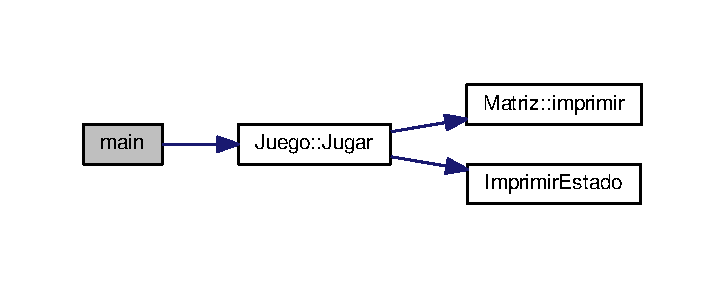
\includegraphics[height=550pt]{main_8cpp_a3c04138a5bfe5d72780bb7e82a18e627_cgraph}
\end{center}
\end{figure}



\section{Matriz.\-cpp File Reference}
\label{_matriz_8cpp}\index{Matriz.\-cpp@{Matriz.\-cpp}}
{\ttfamily \#include \char`\"{}Matriz.\-h\char`\"{}}\\*
{\ttfamily \#include \char`\"{}Lobo.\-h\char`\"{}}\\*
{\ttfamily \#include \char`\"{}Oveja.\-h\char`\"{}}\\*
{\ttfamily \#include \char`\"{}Zorro.\-h\char`\"{}}\\*
{\ttfamily \#include \char`\"{}Raton.\-h\char`\"{}}\\*
Include dependency graph for Matriz.\-cpp\-:
\nopagebreak
\begin{figure}[H]
\begin{center}
\leavevmode
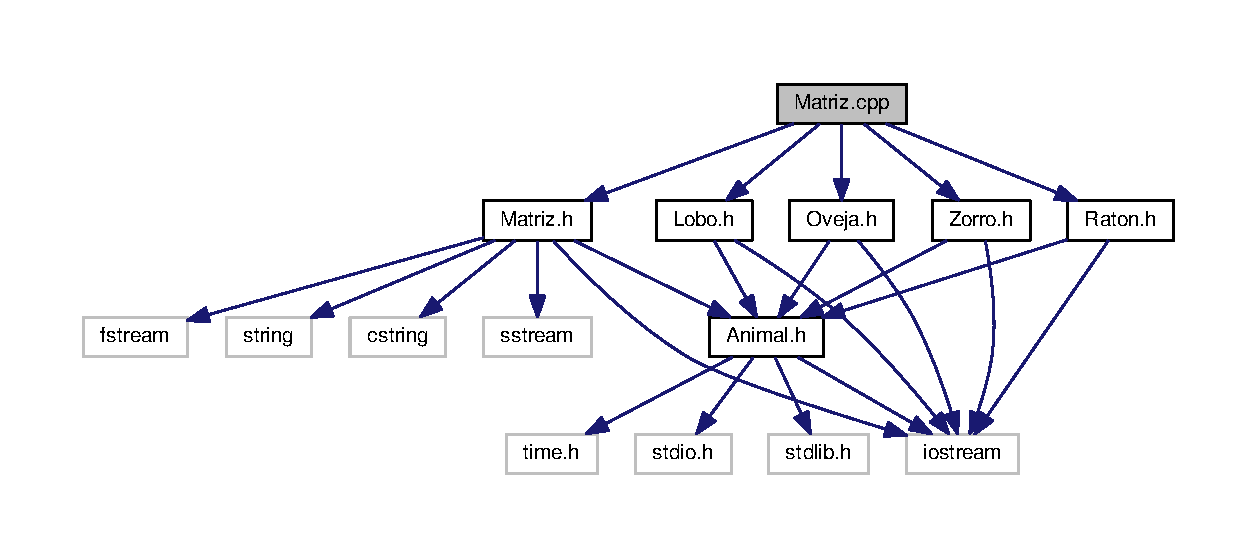
\includegraphics[width=350pt]{_matriz_8cpp__incl}
\end{center}
\end{figure}

\section{Matriz.\-h File Reference}
\label{_matriz_8h}\index{Matriz.\-h@{Matriz.\-h}}
{\ttfamily \#include $<$fstream$>$}\\*
{\ttfamily \#include $<$string$>$}\\*
{\ttfamily \#include $<$cstring$>$}\\*
{\ttfamily \#include $<$sstream$>$}\\*
{\ttfamily \#include $<$iostream$>$}\\*
{\ttfamily \#include \char`\"{}Animal.\-h\char`\"{}}\\*
Include dependency graph for Matriz.\-h\-:
\nopagebreak
\begin{figure}[H]
\begin{center}
\leavevmode
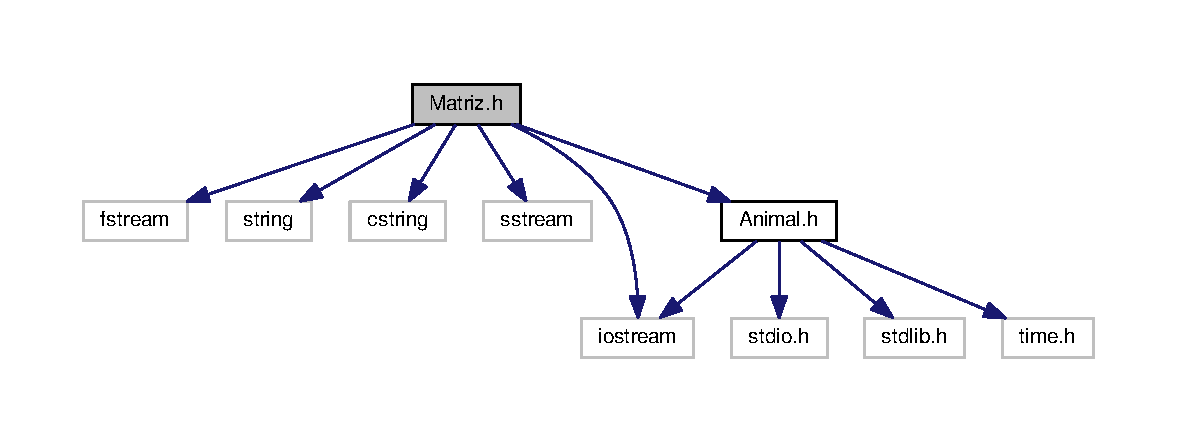
\includegraphics[width=350pt]{_matriz_8h__incl}
\end{center}
\end{figure}
This graph shows which files directly or indirectly include this file\-:
\nopagebreak
\begin{figure}[H]
\begin{center}
\leavevmode
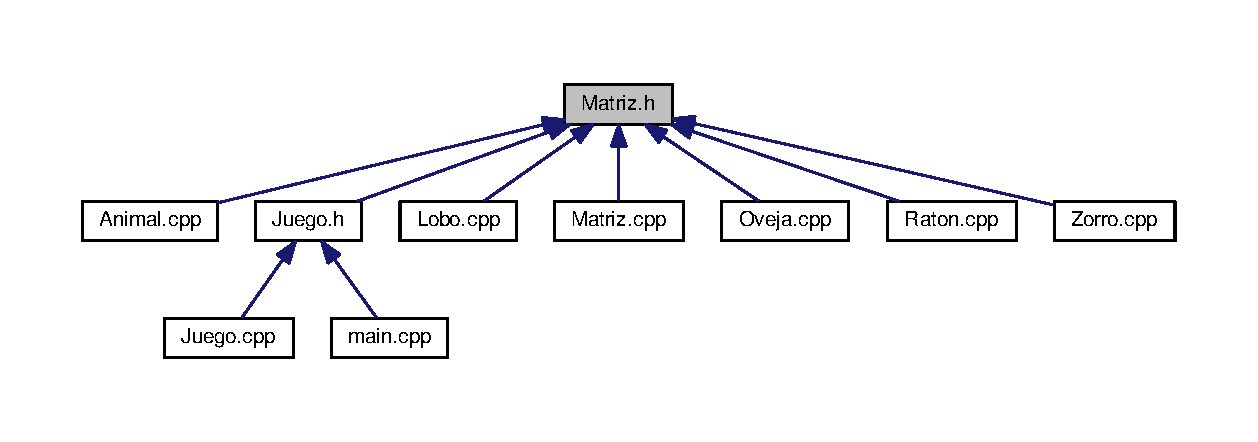
\includegraphics[width=350pt]{_matriz_8h__dep__incl}
\end{center}
\end{figure}
\subsection*{Classes}
\begin{DoxyCompactItemize}
\item 
class {\bf Matriz}
\end{DoxyCompactItemize}
\subsection*{Variables}
\begin{DoxyCompactItemize}
\item 
const int {\bf M\-A\-X\-\_\-\-C\-H\-A\-R\-S\-\_\-\-P\-E\-R\-\_\-\-L\-I\-N\-E} =15
\item 
const int {\bf M\-A\-X\-\_\-\-T\-O\-K\-E\-N\-S\-\_\-\-P\-E\-R\-\_\-\-L\-I\-N\-E} =5
\item 
const char $\ast$const {\bf D\-E\-L\-I\-M\-I\-T\-E\-R} = \char`\"{} \char`\"{}
\end{DoxyCompactItemize}


\subsection{Variable Documentation}
\index{Matriz.\-h@{Matriz.\-h}!D\-E\-L\-I\-M\-I\-T\-E\-R@{D\-E\-L\-I\-M\-I\-T\-E\-R}}
\index{D\-E\-L\-I\-M\-I\-T\-E\-R@{D\-E\-L\-I\-M\-I\-T\-E\-R}!Matriz.h@{Matriz.\-h}}
\subsubsection[{D\-E\-L\-I\-M\-I\-T\-E\-R}]{\setlength{\rightskip}{0pt plus 5cm}const char$\ast$ const D\-E\-L\-I\-M\-I\-T\-E\-R = \char`\"{} \char`\"{}}\label{_matriz_8h_afdcd9e2b2018bb5c8d5781d314c4deb2}
\index{Matriz.\-h@{Matriz.\-h}!M\-A\-X\-\_\-\-C\-H\-A\-R\-S\-\_\-\-P\-E\-R\-\_\-\-L\-I\-N\-E@{M\-A\-X\-\_\-\-C\-H\-A\-R\-S\-\_\-\-P\-E\-R\-\_\-\-L\-I\-N\-E}}
\index{M\-A\-X\-\_\-\-C\-H\-A\-R\-S\-\_\-\-P\-E\-R\-\_\-\-L\-I\-N\-E@{M\-A\-X\-\_\-\-C\-H\-A\-R\-S\-\_\-\-P\-E\-R\-\_\-\-L\-I\-N\-E}!Matriz.h@{Matriz.\-h}}
\subsubsection[{M\-A\-X\-\_\-\-C\-H\-A\-R\-S\-\_\-\-P\-E\-R\-\_\-\-L\-I\-N\-E}]{\setlength{\rightskip}{0pt plus 5cm}const int M\-A\-X\-\_\-\-C\-H\-A\-R\-S\-\_\-\-P\-E\-R\-\_\-\-L\-I\-N\-E =15}\label{_matriz_8h_a3b95e0254661c995b723a9b150a821c1}
\index{Matriz.\-h@{Matriz.\-h}!M\-A\-X\-\_\-\-T\-O\-K\-E\-N\-S\-\_\-\-P\-E\-R\-\_\-\-L\-I\-N\-E@{M\-A\-X\-\_\-\-T\-O\-K\-E\-N\-S\-\_\-\-P\-E\-R\-\_\-\-L\-I\-N\-E}}
\index{M\-A\-X\-\_\-\-T\-O\-K\-E\-N\-S\-\_\-\-P\-E\-R\-\_\-\-L\-I\-N\-E@{M\-A\-X\-\_\-\-T\-O\-K\-E\-N\-S\-\_\-\-P\-E\-R\-\_\-\-L\-I\-N\-E}!Matriz.h@{Matriz.\-h}}
\subsubsection[{M\-A\-X\-\_\-\-T\-O\-K\-E\-N\-S\-\_\-\-P\-E\-R\-\_\-\-L\-I\-N\-E}]{\setlength{\rightskip}{0pt plus 5cm}const int M\-A\-X\-\_\-\-T\-O\-K\-E\-N\-S\-\_\-\-P\-E\-R\-\_\-\-L\-I\-N\-E =5}\label{_matriz_8h_a72dd0d57927dd2f5568e5160f7940fed}

\section{Oveja.\-cpp File Reference}
\label{_oveja_8cpp}\index{Oveja.\-cpp@{Oveja.\-cpp}}
{\ttfamily \#include \char`\"{}Oveja.\-h\char`\"{}}\\*
{\ttfamily \#include \char`\"{}Matriz.\-h\char`\"{}}\\*
Include dependency graph for Oveja.\-cpp\-:
\nopagebreak
\begin{figure}[H]
\begin{center}
\leavevmode
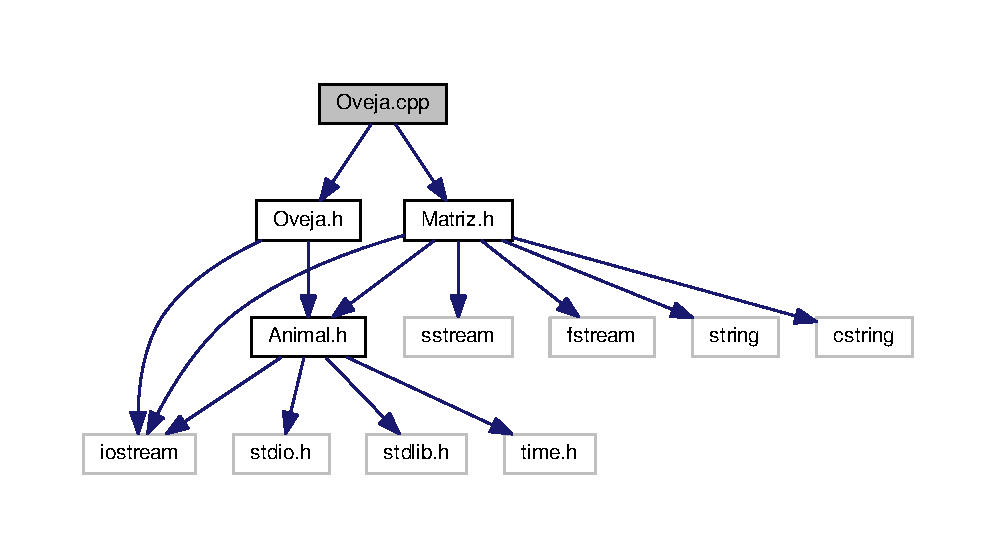
\includegraphics[width=350pt]{_oveja_8cpp__incl}
\end{center}
\end{figure}

\section{Oveja.\-h File Reference}
\label{_oveja_8h}\index{Oveja.\-h@{Oveja.\-h}}
{\ttfamily \#include $<$iostream$>$}\\*
{\ttfamily \#include \char`\"{}Animal.\-h\char`\"{}}\\*
Include dependency graph for Oveja.\-h\-:
\nopagebreak
\begin{figure}[H]
\begin{center}
\leavevmode
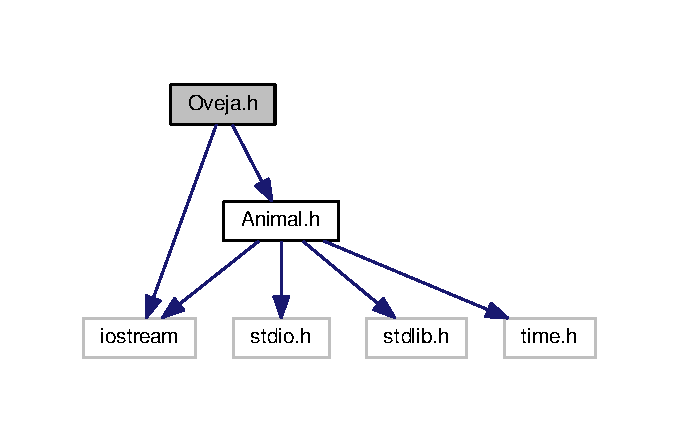
\includegraphics[width=326pt]{_oveja_8h__incl}
\end{center}
\end{figure}
This graph shows which files directly or indirectly include this file\-:
\nopagebreak
\begin{figure}[H]
\begin{center}
\leavevmode
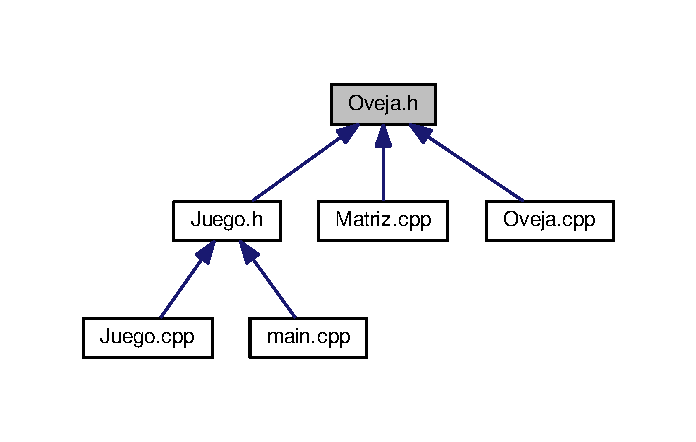
\includegraphics[width=334pt]{_oveja_8h__dep__incl}
\end{center}
\end{figure}
\subsection*{Classes}
\begin{DoxyCompactItemize}
\item 
class {\bf Oveja}
\end{DoxyCompactItemize}

\section{Raton.\-cpp File Reference}
\label{_raton_8cpp}\index{Raton.\-cpp@{Raton.\-cpp}}
{\ttfamily \#include \char`\"{}Raton.\-h\char`\"{}}\\*
{\ttfamily \#include \char`\"{}Matriz.\-h\char`\"{}}\\*
Include dependency graph for Raton.\-cpp\-:
\nopagebreak
\begin{figure}[H]
\begin{center}
\leavevmode
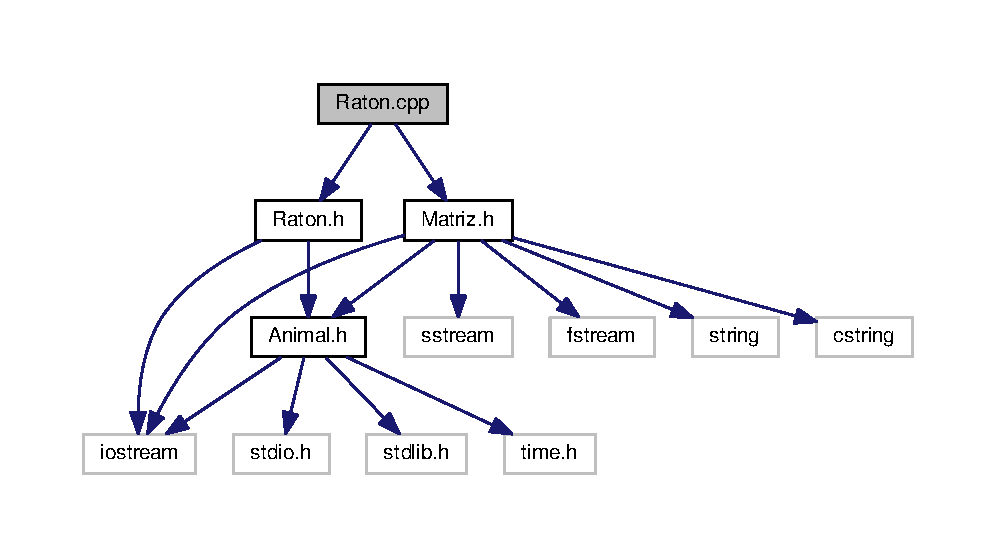
\includegraphics[width=350pt]{_raton_8cpp__incl}
\end{center}
\end{figure}

\section{Raton.\-h File Reference}
\label{_raton_8h}\index{Raton.\-h@{Raton.\-h}}
{\ttfamily \#include $<$iostream$>$}\\*
{\ttfamily \#include \char`\"{}Animal.\-h\char`\"{}}\\*
Include dependency graph for Raton.\-h\-:
\nopagebreak
\begin{figure}[H]
\begin{center}
\leavevmode
\includegraphics[width=326pt]{_raton_8h__incl}
\end{center}
\end{figure}
This graph shows which files directly or indirectly include this file\-:
\nopagebreak
\begin{figure}[H]
\begin{center}
\leavevmode
\includegraphics[width=335pt]{_raton_8h__dep__incl}
\end{center}
\end{figure}
\subsection*{Classes}
\begin{DoxyCompactItemize}
\item 
class {\bf Raton}
\end{DoxyCompactItemize}

\section{Zorro.\-cpp File Reference}
\label{_zorro_8cpp}\index{Zorro.\-cpp@{Zorro.\-cpp}}
{\ttfamily \#include \char`\"{}Zorro.\-h\char`\"{}}\\*
{\ttfamily \#include \char`\"{}Matriz.\-h\char`\"{}}\\*
Include dependency graph for Zorro.\-cpp\-:
\nopagebreak
\begin{figure}[H]
\begin{center}
\leavevmode
\includegraphics[width=350pt]{_zorro_8cpp__incl}
\end{center}
\end{figure}

\section{Zorro.\-h File Reference}
\label{_zorro_8h}\index{Zorro.\-h@{Zorro.\-h}}
{\ttfamily \#include $<$iostream$>$}\\*
{\ttfamily \#include \char`\"{}Animal.\-h\char`\"{}}\\*
Include dependency graph for Zorro.\-h\-:
\nopagebreak
\begin{figure}[H]
\begin{center}
\leavevmode
\includegraphics[width=326pt]{_zorro_8h__incl}
\end{center}
\end{figure}
This graph shows which files directly or indirectly include this file\-:
\nopagebreak
\begin{figure}[H]
\begin{center}
\leavevmode
\includegraphics[width=331pt]{_zorro_8h__dep__incl}
\end{center}
\end{figure}
\subsection*{Classes}
\begin{DoxyCompactItemize}
\item 
class {\bf Zorro}
\end{DoxyCompactItemize}

%--- End generated contents ---

% Index
\newpage
\phantomsection
\addcontentsline{toc}{chapter}{Index}
\printindex

\end{document}
